\documentclass[hidelinks, a4paper,12pt]{article}
\usepackage{ amsmath, amssymb}
\usepackage{graphicx}
\usepackage{color,amsmath,graphics,graphicx}
\usepackage{amsfonts} % replace subfigure with subcaption instead 
\usepackage{mathrsfs,hyperref}
\usepackage{latexsym,amsmath,enumerate,amsbsy,amsthm,verbatim,enumitem}
\usepackage{amstext,amsopn}
\usepackage{makeidx} 
\textwidth = 415pt

%==============================================
\usepackage{fontspec}
\usepackage{xunicode}
\usepackage{xltxtra}
\defaultfontfeatures{Scale=1.23}
\XeTeXlinebreaklocale “th_TH” % สำหรับตัดคำ
\setmainfont[Scale=1.23]{THSarabunNew}
%==============================================
%%%%%%%%%%%%%%% THEOREM Environments %%%%%%%%%% 
\newtheorem{theorem}{ทฤษฎีบท}[section]						%
\newtheorem{lemma}[theorem]{บทตั้ง}						%
\newtheorem{conjecture}[theorem]{บทคาดการณ์}				%
\newtheorem{definition}[theorem]{บทนิยาม}					%
\newtheorem{remark}[theorem]{หมายเหตุ}						%
\newtheorem{proposition}[theorem]{ประพจน์}					%
\newtheorem{corollary}[theorem]{บทแทรก}					%
\numberwithin{equation}{section}							%
\newtheorem{example}[theorem]{ตัวอย่าง}						%
%\newtheorem{exercise}{แบบฝึกหัด}[chapter]	
%\renewcommand{\chaptername}{บทที่}
\renewcommand\tablename{ตารางที่}
\renewcommand\figurename{รูปที่}
\renewcommand{\contentsname}{สารบัญ}						%
%\renewcommand{\bibname}{บรรณานุกรม}						% 
\renewcommand{\indexname}{ดรรชนี}					%
\counterwithin{figure}{section}
\numberwithin{equation}{section}		
%%%%%%%%%%%%%%%%%%%%%%%%%%%%%%%%%%%%%%%%%%%%%%%
% addition mod
\usepackage{subcaption,float,framed,hyperref}
\usepackage[ruled]{algorithm2e}
% =============

\begin{document}
	{\begin{center}
			\textbf{Report Progress}\\
			\vspace{0.5cm}
			\textbf{Division of Applied Mathematics, Department of Mathematics}\\
			\vspace{0.5cm}
			\textbf{Faculty of Science, Silpakorn University}
		\end{center}}
		{
			\vspace{0.5cm}
			\flushleft{Date : { 23 พฤศจิกายน 2561 } \hfill{ }}
			\flushleft{Advisor : { ผู้ช่วยศาสตราจารย์ ดร.นพดล  ชุมชอบ}}\\
			\flushleft{Student : {นายภัคพล พงษ์ทวี รหัส  07580028}
			\vspace{1cm}
		}
		
		
		% Here the project title
		{\textbf{\begin{flushleft}Project Title : ขั้นตอนวิธีเชิงตัวเลขชนิดใหม่สำหรับการต่อเติมภาพที่ใช้การแปรผันรวมกับการประยุกต์สำหรับซ่อมแซมภาพจิตรกรรมไทยโบราณและการลบบทบรรยายจากอนิเมะ \\
				(A new numerical algorithm for TV-based image inpainting with its applications for restoring ancient Thai painting images and removing subtitles from animes)
			\end{flushleft}
		}}
		\thispagestyle{empty}
	\section{ที่มาและความสำคัญ}
	\hspace{1cm} ในปัจจุบันการใช้ภาพดิจิตัล (digital images) ในสังคมเครือข่ายได้รับความนิยมอย่างแพร่หลาย เนื่องจากโทรศัพท์เคลื่อนที่มีราคาถูกลงแต่มีความสามารถที่ชาญฉลาด สามารถทำหน้าที่ได้ตั้งแต่การเป็นกล้องดิจิตัลคอมแพค (compact digital camera)  คุณภาพดีให้ภาพดิจิตัลที่มีความคมชัดสูงจนไปถึงการทำหน้าที่ดังเช่นเครื่องคอมพิวเตอร์ส่วนบุคคลที่สามารถเชื่อมต่อกับระบบเครือข่ายไร้สายเพื่อรับส่งภาพดิจิตัลในสังคมเครือข่ายด้วยความสะดวกและรวดเร็ว 
	
	\hspace{1cm} นอกจากภาพดิจิตัลจะได้รับจากการถ่ายภาพด้วยโทรศัพท์เคลื่อนที่แล้ว ภาพดิจิตัลยังได้รับการถ่ายภาพด้วยกล้องดีเอสแอลอาร์ หรือ กล้องสะท้อนเลนส์เดี่ยวแบบดิจิตัล (digital single lens reflex camera) กล้องโทรทรรศน์ (หรือ กล้องดูดาว) หรือ เครื่องมือสร้างภาพถ่ายทางการแพทย์ (medical imaging device) 
	
	\hspace{1cm} โดยทั่วไปภาพดิจิตัลจะได้รับการประมวลผลภาพก่อนนำไปใช้งานเพื่อให้สามารถใช้ข้อมูลที่ปรากฎบนภาพได้ตรงวัตถุประสงค์ของการใช้งานมากที่สุด ตัวอย่างเช่น ภาพบุคคล (portrait) อาจจำเป็นต้องได้รับการกำจัดสัญญาณรบกวนออกจากภาพและ/หรือปรับเพิ่มความละเอียดข้อมูลของความเข้มของสีและความสว่างของสีบนบริเวณใบหน้าก่อนนำภาพไปใช้งานเพื่อจัดทำต้นฉบับวารสารหรือหนังสือของสำนักพิมพ์ เป็นต้น  
	
	\hspace{1cm} การต่อเติมภาพ (image inpainting) เป็นวิธีการประมวลผลภาพชนิดหนึ่งมีเป้าหมายเพื่อซ่อมแซมภาพด้วยการต่อเติมข้อมูลของความเข้มของสีบนบริเวณที่กำหนด (ต่อไปจะเรียกบริเวณนี้ว่าโดเมนต่อเติม (inpainting domain)) โดยอาศัยข้อมูลของความเข้มของสีที่ปรากฏในภาพ ตัวอย่างเช่น 
	กำหนดให้รูปที่ \ref{fig1} (a) แสดงภาพที่ต้องการซ่อมแซมระดับความเข้มของสีบนบริเวณแท่งวัตถุรูปร่างสี่เหลี่ยมสีขาว การต่อเติมภาพดังกล่าวจะเริ่มด้วยการกำหนดให้บริเวณแท่งวัตถุรูปร่างสี่เหลี่ยมสีขาวเป็นโดเมนการต่อเติมดังรูปที่ \ref{fig1} (b) จากนั้นภาพที่ได้รับการซ่อมแซมหรือภาพที่ได้รับการต่อเติม (restored or inpainted image) ซึ่งแสดงในรูปที่ \ref{fig1} (c) ได้มาจากขั้นตอนวิธีการต่อเติมภาพ (inpainting algorithm) ซึ่งได้รับการออกแบบเพื่อนำข้อมูลที่ปรากฎบนภาพในบริเวณใกล้เคียงกับขอบของโดเมนต่อเติมมาซ่อมแซมภาพ 
	
	\begin{figure}[H]
		\centering
		\begin{subfigure}{0.3\linewidth}
			\centering
			
\includegraphics[width=0.8\linewidth]{images/grayscale_inpaint/toinpaint.png}
			\caption{ภาพที่ต้องการซ่อมแซม}
		\end{subfigure}
		\begin{subfigure}{0.3\linewidth}
			\centering
			
\includegraphics[width=0.8\linewidth]{images/grayscale_inpaint/inpaintdomain.png}
			\caption{โดเมนต่อเติม}
		\end{subfigure}
		\begin{subfigure}{0.3\linewidth}
			\centering
			
\includegraphics[width=0.8\linewidth]{images/grayscale_inpaint/result_splitbergman.png}
			\caption{ภาพที่ได้รับการซ่อมแซม}
		\end{subfigure}
		\caption{ตัวอย่างการซ่อมแซมภาพ; (a) ภาพที่ต้องการซ่อมแซม; (b) โดเมนต่อเติม; (c) ภาพที่ได้รับการซ่อมแซม}
		\label{fig1}
	\end{figure}
	
	\hspace{1cm} เท่าที่ผู้วิจัยศึกษาและค้นคว้ามาจนถึงขณะนี้ ผู้วิจัยพบว่าการต่อเติมภาพมักนิยมนำไปใช้งานสำหรับการปรับแต่งความสวยงามของภาพบุคคลที่ถ่ายจากโทรศัพท์เคลื่อนที่ เช่น การลบร่องรอยของรอยตีนกา การลบร่องรอยแผลเป็นที่เกิดจากสิวเสี้ยน การลดร่องรอยของความชรา หรือ การเพิ่มความใสและความเนียนของสีผิวบนบริเวณใบหน้าผ่านโปรแกรมแอปพลิเคชันแต่งรูปภาพที่มีอยู่ในแอปสโตร์ (App Store) หรือ กูเกิ้ลเพลย์ (Google Play) เป็นต้น 
	
	\subsection{การซ่อมแซมภาพจิตรกรรมไทยโบราณ}
	
	\hspace{1cm} ภาพจิตรกรรมไทย คือ ภาพเขียนที่มีเอกลักษณ์ความเป็นศิลปะไทยซึ่งโดดเด่นและแตกต่างจากภาพเขียนของชนชาติอื่น ในอดีต  ช่างไทยได้สร้างสรรค์ลวดลายและสีสันบนภาพวาดเพื่อสะท้อนประเพณีและวัฒนธรรมในสังคมไทยที่เกี่ยวกับศาสนา ประวัติศาสตร์ โบราณคดี ชีวิตความเป็นอยู่ วัฒนธรรมการแต่งกาย ตลอดจนการแสดงการเล่นพื้นเมืองต่าง ๆ ของแต่ละยุคสมัย 
	
	\hspace{1cm} อย่างไรก็ตาม ภาพจิตรกรรมไทยจำนวนไม่น้อยที่เสื่อมสลายตามกาลเวลา และรอคอยการซ่อมแซมจากช่างในสมัยปัจจุบันที่ต้องไม่สร้างความเสียหายให้กับภาพเขียนเพิ่มขึ้นมากกว่าเดิม  ที่ผ่านมาภาพที่ผ่านการซ่อมแซมมาแล้วจำนวนไม่น้อยได้รับความเสียหายหลังจากการซ่อมแซม ถึงแม้สภาพโดยรวมของภาพจิตรกรรมเดิมยังคงอยู่ แต่รายละเอียดในตัวภาพเขียนได้เปลี่ยนไป ก่อให้เกิดความเสียหายที่ประเมินค่าไม่ได้ 
	
	\hspace{1cm} การซ่อมแซมภาพจิตรกรรมไทยโบราณโดยใช้การต่อเติมภาพเป็นขั้นตอนของการซ่อมแซมแบบหนึ่งซึ่งไม่ก่อให้เกิดความเสียหายใด ๆ กับภาพเดิม เนื่องจากเป็นการซ่อมแซมโดยการใช้ขั้นตอนวิธีเชิงตัวเลขบนภาพดิจิตัลซึ่งเป็นสำเนาของภาพเดิม ด้วยเหตุผลดังกล่าว ผู้วิจัยได้เล็งเห็นว่าการซ่อมแซมภาพจิตรกรรมไทยโบราณมีความจำเป็นเร่งด่วน เนื่องจากภาพที่ได้รับการซ่อมแซมด้วยการต่อเติมภาพสามารถนำไปใช้ประกอบการตัดสินใจเพื่อวางแผนก่อนการลงมือซ่อมแซมภาพเขียนจริงได้ นอกจากนี้ ขั้นตอนวิธีการต่อเติมภาพสามารถนำไปใช้สร้างแอปพลิเคชันบนโทรศัพท์เคลื่อนที่เพื่อในไปใช้เป็นข้อมูลในการเข้าชมภาพเขียนเดิมที่ยังไม่ได้รับการซ่อมแซมและภาพเขียนที่ได้รับการซ่อมแซมโดยวิธีการทางคณิตศาสตร์จากแอปพลิเคชันที่พัฒนาขึ้น
	
	\hspace{1cm} รูปที่ \ref{fig2} แสดงตัวอย่างภาพจิตรกรรมไทย\footnote{ภาพถ่ายที่วัดภูมินทร์ อำเภอเมือง จังหวัดน่าน; ภาพจาก http://topicstock.pantip.com/camera/topicstock/2009/02/O7514399/O7514399.html สืบค้นเมื่อวันที่ 23 กันยายน 2561} ที่ต้องได้รับการซ่อมแซมบนบริเวณแขนเสื้อของรูปวาดผู้ชายที่มีส่วนของสีแดงเดิมหลุดหายไป ทั้งนี้ในการซ่อมแซมภาพโดยการต่อเติมภาพ เราจะเริ่มด้วยการสร้างโดเมนต่อเติมบนบริเวณสีพื้นผิวปูนที่แขนเสื้อ จากนั้นจึงนำขั้นตอนวิธีการต่อเติมภาพเพื่อซ่อมแซมภาพบริเวณนั้นให้เป็นสีแดง 
	
	\begin{figure}[h]
		\[
		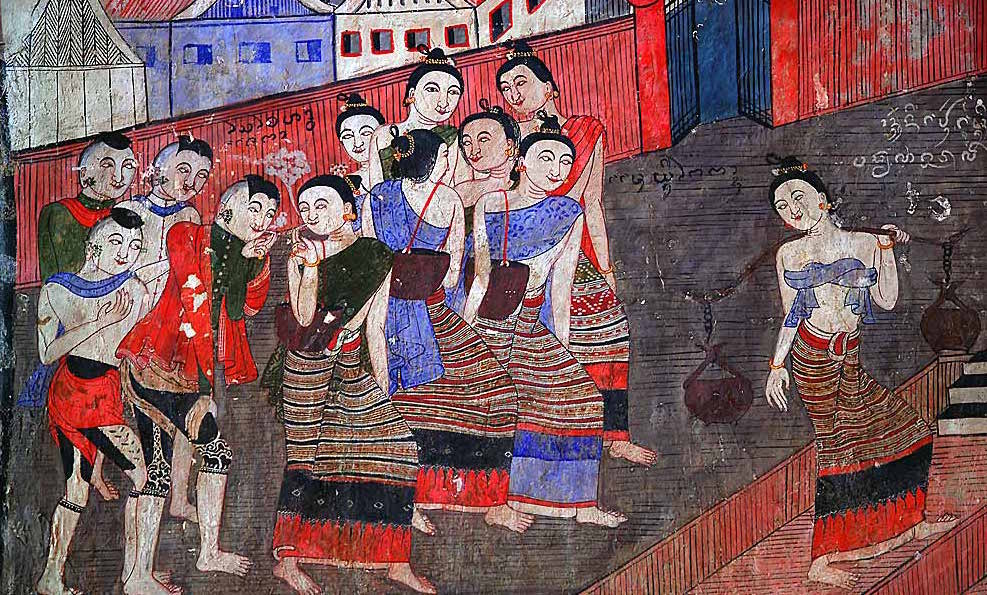
\includegraphics[width=0.6\linewidth]{images/show_peicewise/fig2a.jpg}
		\]
		\caption{ภาพจิตรกรรมไทยที่วัดภูมินทร์ อำเภอเมือง จังหวัดน่าน}
		\label{fig2}
	\end{figure}
	
	
	\subsection{การลบบทบรรยายบนอนิเมะ}
	\hspace{1cm}อนิเมะคือวิดีโอภาพวาดการ์ตูนสไตล์ญี่ปุ่นซึ่งเป็นที่นิยมของเยาวชนไทย ในการรับชมอนิเมะ แม้ว่าเยาวชนไทยสามารถรับชมด้วยบทพากย์เสียงภาษาไทย แต่ก็สูญเสียอรรถรสของการรับชมจากบทบรรยายแบบแข็ง\footnote{บทยรรยายที่ไม่สามารถปิดหรือเปิดได้} (hardsub) ที่เป็นภาษาต่างประเทศในบริเวณด้านล่างของจอภาพ ในการซ่อมแซม\\อนิเมะด้วยการลบบทบรรยายภาษาต่างประเทศจึงเป็นงานที่ยุ่งยากและท้าท้ายมาก เนื่องจาก
	\begin{itemize}
		\item [(1)] อนิเมะเป็นวิดีโอซึ่งแสดงผลประมาณ 24 เฟรม(ภาพ)ต่อวินาที
		\item [(2)] แต่ละเฟรมอาจมีหรืออาจไม่มีบทบรรยายก็ได้
		\item [(3)] แต่ละเฟรมอาจมีหรืออาจไม่มีบทบรรยายเดียวกันก็ได้
		\item [(4)] แต่ละเฟรมเป็นการแสดงผลภาพสีที่มีระดับความคมชัดสูง (high definition) ขนาดมากถึง $1920\times1080$ พิกเซล
	\end{itemize}
	ด้วยความท้าทายข้างต้น การพัฒนาขั้นตอนวิธีการต่อเติมภาพที่สามารถกำหนดโดเมนต่อเติมเชิงอัตโนมัติให้กับแต่ละเฟรมและประมวลผลได้แม่นยำจนการลบบทบรรยายสามารถทำงานได้แบบเรียลไทม์จึงเป็นสิ่งจำเป็นที่หลีกเลี่ยงไม่ได้
	
	\hspace{1cm} รูปที่ \ref{fig3} แสดงตัวอย่าง 1 เฟรมของอนิเมะที่มีบทบรรยายแบบแข็ง\footnote{ภาพจาก https://www.samehadaku.tv/2018/07/grand-blue-episode-1-subtitle-indonesia.html สืบค้นเมื่อวันที่ 23 กันยายน 2561} ที่ต้องซ่อมแซมด้วยการลบบทบรรยายออก  ทั้งนี้ในการลบบทบรรยายออกจากเฟรมโดยใช้การต่อเติมภาพ เราจะเริ่มด้วยการสร้างโดเมนต่อเติมแบบอัตโนมัติในบริเวณบทบรรยาย จากนั้นจึงนำขั้นตอนวิธีการต่อเติมภาพแบบเร็วเพื่อลบบทบรรยายออกจากเฟรม 
	
	\begin{figure}[h]
		\[
		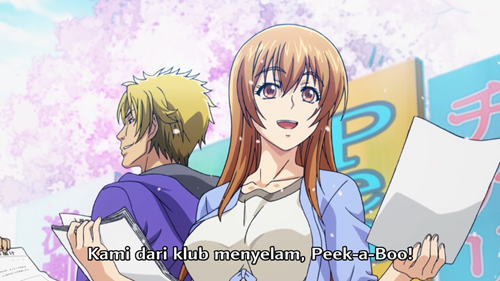
\includegraphics[width=0.6\linewidth]{images/show_peicewise/fig3.png}
		\]
		\caption{1 เฟรมของอนิเมะที่มีบทบรรยายแบบแข็ง}
		\label{fig3}
	\end{figure}
	
	\hspace{1cm} โครงการวิจัยนี้ ผู้วิจัยมีเป้าหมายสำคัญคือการพัฒนาขั้นตอนวิธีการต่อเติมภาพแบบเร็วและแม่นยำชนิดใหม่เพื่อนำไปใช้สำหรับซ่อมแซมภาพจิตรกรรมไทยและการลบบทบรรยายออกจากอนิเมะ


\section{วรรณกรรมและทฤษฎีบทที่เกี่ยวข้อง} 
\hspace{1cm} ในการกล่าวถึงขั้นตอนวิธีการต่อเติมภาพ จะเริ่มต้นด้วยการกล่าวทบทวนเกี่ยวกับการต่อเติมภาพเฉดสีเทา (grayscale image) ก่อน ดังนี้

\hspace{1cm} ให้ $\Omega \subset \mathbb{R}^2$ แทนโดเมนภาพ (image domain) $D \subset \mathbb{R}^2$ แทนโดเมนต่อเติม (ดูรูปที่ \ref{fig4}) และ $V \subset [0,\infty)$ 

\hspace{1cm} ให้ $ u: \Omega \rightarrow V,\ z: \Omega \rightarrow V$ แทนภาพที่ได้รับการซ่อมแซมและภาพที่ต้องการซ่อมแซม ตามลำดับ

\hspace{1cm} ในที่นี้ $ \mathbf{x} = (x,y) \in \Omega $ แทนพิกัดทางกายภาพ (physical position) ของภาพ และ $ u(\mathbf{x}) \in V $ แทนระดับความเข้มของภาพ (image intensity) ที่ $ \mathbf{x} $ และ $ \Omega $ มีรูปร่างสี่เหลี่ยม 

\hspace{1cm} นอกจากนี้เราสามารถสมมติได้โดยไม่เสียหลักการสำคัญว่า $ \Omega = [1,n]^2 $ และ $ V = [0,1] $ เมื่อ $n>0$ เป็นจำนวนเต็มบวก ทั้งนี้ เราจะเรียกภาพ $u,z$ ที่นิยามข้างต้นว่าภาพเฉดสีเทา
\begin{figure}[H]
	\centering
	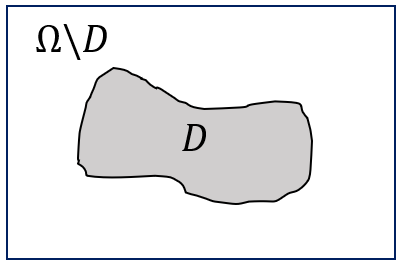
\includegraphics[width=0.4\linewidth]{images/sample-domain.png}
	\caption{$D$ แทนโดเมนต่อเติม}
	\label{fig4}
\end{figure}

\subsection{ตัวแบบการต่อเติมภาพเฉดสีเทาที่ใช้การแปรผันรวม}\label{inpaint-model-grayscale}

\hspace{1cm} ในการต่อเติมภาพเฉดสีเทา Chan และ Shen \cite{ref:rof-inpaint-chan-shen} ได้นำเสนอตัวแบบเชิงการแปรผัน (variational model) ที่ใช้เร็กกิวลาร์ไรซ์เซชันแบบการแปรผันรวม (Total variation based regularization) โดยพัฒนาต่อจากตัวแบบ ROF สำหรับการกำจัดสัญญาณรบกวน \cite{ref:ROF-template} ซึ่งตัวแบบเชิงการแปรผันนี้กำหนดโดย
\begin{align}
\min_{u} \{ \mathcal{J}(u) = \frac{1}{2} \int_{\Omega}\lambda (u-z)^2 d\Omega +  \int_{\Omega}  |\nabla u|  d\Omega \}
\label{e1}
\end{align}
เมื่อ 
\begin{align}
\lambda=\lambda(\mathbf{x}) = \left \{ \begin{array}{ll}  \lambda_0, & x \in \Omega \textbackslash D \\ 0, & x \in D  \end{array} \right . 
\label{e2}
\end{align}
แทนพารามิเตอร์เร็กกิวลาร์ไรซ์เซชัน (regularization parameter) และ $\lambda_0 >0$

\hspace{1cm} โดยแคลคูลัสของการแปรผัน (Calculus of variations) จะได้สมการออยเลอร์ลากรางจ์ที่เกี่ยวข้องกับ (\ref{e1}) เป็น 
\begin{align}
\left \{ \begin{array}{ll}  - \nabla \cdot  \Big( \dfrac{\nabla u}{|\nabla u|} \Big) + \lambda (u-z) = 0,  & \hspace{1cm} \mathbf{x} \in (1,n)^2 \\ \dfrac{\partial u}{\partial \boldsymbol{n}} = 0, & \hspace{1cm} x \in \partial \Omega \end{array} \right . 
\label{e3}
\end{align}
เมื่อ $\boldsymbol{n}$ แทนเวกเตอร์หน่วยที่ตั้งฉากกับของของภาพ

\hspace{1cm} ต่อไปจะกล่าวทบทวนวิธีการเชิงตัวเลขสำหรับแก้สมการเชิงอนุพันธ์ย่อยใน (\ref{e3}) 

\begin{itemize}
	\item [(1)] วิธีการเดินเวลาแบบชัดแจ้ง (explicit time marching method) 
	
	คณะวิจัย \cite{ref:ROF-template} ได้แนะนำวิธีการเชิงตัวเลขสำหรับการกำจัดสัญญาณรบกวนโดยใช้วิธีการเดินเวลาแบบชัดแจ้ง ซึ่งสามารถประยุกต์เป็นวิธีเชิงตัวเลขสำหรับการต่อเติมภาพได้ดังนี้
	
	\hspace{1cm} เริ่มจากการแนะนําตัวแปรเวลาสังเคราะห์ (time artificial variable) จากนั้นหาคําตอบแบบสภาวะคงตัว (steady-state solution) ในขณะที่ $t\rightarrow \infty$ ของสมการเชิงอนุพันธ์ย่อยไม่เป็นเชิงเส้นที่ขึ้นอยู่กับเวลา 
	\begin{align}
	u(\mathbf{x},t_{k+1})=u(\mathbf{x},t_{k})+\tau\left(\nabla \cdot\left(\dfrac{\nabla u (\mathbf{x},t_k)}{| \nabla u (\mathbf{x},t_k) | }\right) + \lambda(\mathbf{x})(u (\mathbf{x},t_k)-z(\mathbf{x})) \right),\ u(\mathbf{x},t_0)=z
	\label{e4}
	\end{align}
	เมื่อ $t_k=t_0+k\tau\ (\tau>0)$  แทนขั้นเวลาที่ $k$ และ $t_0=0$ แทนขั้นเวลาเริ่มต้น
	
	\item [(2)] วิธีการทำซ้ำแบบจุดตรึง (fixed-point iteration method)
	
	คณะวิจัย \cite{ref:FixpointSolver} ได้แนะนำวิธีการเชิงตัวเลขสำหรับการกำจัดสัญญาณรบกวนโดยใช้วิธีการทำซ้ำแบบจุดตรึง ซึ่งสามารถประยุกต์เป็นวิธีเชิงตัวเลขสำหรับการต่อเติมภาพได้ดังนี้
	
	\hspace{1cm} เริ่มจากแนะนำดัชนีการทำซ้ำแบบจุดตรึง $\nu=0,1,2,\cdots$ และนิยามรูปแบบการทำซ้ำโดย
	\begin{align}
	- \nabla\cdot\left(\dfrac{\nabla u^{[\nu+1]}}{{| \nabla u |}^{[v]} }\right) + \lambda(u^{[\nu+1]}-z)  = 0,\ u^{[0]}=z
	\label{e5}
	\end{align}
\end{itemize}

\hspace{1cm} เนื่องจาก $\tfrac{1}{| \nabla u |}=\tfrac{1}{\sqrt{u_x^2+u_y^2}} \rightarrow \infty$ ในบริเวณที่ $u$ มีความเข้มสีเป็นเอกพันธ์ุ ($u(\mathbf{x})=$ ค่าคงตัว) เพื่อหลีกเลี่ยงปัญหาเชิงตัวเลขจะเกิดขึ้นใน (\ref{e4}) และ (\ref{e5}) เราจะใช้ 
\begin{align*}
|\nabla u| \approx| \nabla u |_\beta=\sqrt{u_x^2+u_y^2+\beta},\ 0< \beta \ll 1
 \end{align*}
จึงทำให้สามารถเขียน วิธีเดินเวลาแบบชัดแจ้งสำหรับภาพเฉดเทาเป็นขั้นตอนวิธีได้ดังนี้ 
\begin{algorithm}[H]
	\caption{Explicit time marching gray-scale solver}
	\KwIn{
		\\
		\hspace{1cm} $u$ is image which is damaged image \\
		\hspace{1cm} $\lambda$ is regularization parameter which has explain in equation (\ref{e2}) \\
		\hspace{1cm} $\beta$ is positive rational number which is use to avoid devide by zero \\
		\hspace{1cm} $\tau$ is positive rational number which is marching parameter \\
		\hspace{1cm} $N$ is positive interger  which is number of maximum loop iteration \\
		\hspace{1cm} $\varepsilon$ is positive rational number  which is expected relative error \\
	}
	\KwOut{inpainted image}    
	\SetKwFunction{FMain}{ExplictTimeMarchingInpaint}
	\SetKwProg{Fn}{Function}{:}{}
	\Fn{\FMain{$u, \lambda, \tau, \beta, N, \varepsilon$}}{
		\textbf{initialize}
		$i = 0$ 
		$z = u$\\
		\While{$ i < N $ \textbf{and} $err > \varepsilon$}{
			$u^{old} = u$\\
			$u = u + \tau\left(\nabla \cdot\left(\dfrac{\nabla u}{\sqrt{u_x^2 + u_y^2+ \beta}}\right) + \lambda(u-z) \right)$ \\ 		
			$err = \frac{||u-u^{old}||}{||u||}$ \\
			$ i = i + 1 $
		}
		\textbf{return} $ u $ 
	}
\end{algorithm}

\clearpage
และจะสามารถเขียน ขั้นตอนวิธีจุดตรึงสำหรับภาพเฉดเทาเป็นขั้นตอนวิธีได้ดังนี้ 
\begin{algorithm}[H]
	\caption{Fixed point gray-scale solver}
	\KwIn{
		\\
		\hspace{1cm} $u$ is image which is damaged image \\
		\hspace{1cm} $\lambda$ is regularization parameter which has explain in equation (\ref{e2}) \\
		\hspace{1cm} $\beta$ is positive rational number which is use to avoid devide by zero \\
		\hspace{1cm} $N_{gs}$ is positive integer which is number of gauss seidel iteration \\
		\hspace{1cm} $N$ is positive interger  which is number of maximum loop iteration \\
		\hspace{1cm} $\varepsilon$ is positive rational number  which is expected relative error \\
	}
	\KwOut{inpainted image}    
	\SetKwFunction{FMain}{FixedPointInpaint}
	\SetKwProg{Fn}{Function}{:}{}
	\Fn{\FMain{$u, \lambda, \beta, N_{gs},  N, \varepsilon$}}{		
		\textbf{initialize} $i=0$\\
		$u = z$ \\
		\While{$ i < N $ \textbf{and} $err > \varepsilon$}{
			$ u^{old} = u$ \\
			$u = InnerFixedPointInpaint(u, z, \lambda, \beta, N_{gs})$\\
			$err = \frac{||u-u^{old}||}{||u||}$		
			$ i = i + 1 $
		}
		\textbf{return} $ u $ 
	}
	\SetKwFunction{FMain}{InnerFixedPointInpaint}
	\Fn{\FMain{$u, z, \lambda, \beta, N_{gs}$}}{
		\textbf{initialize} $k = 0$\\
		compute $D(u) = \frac{1}{\sqrt{u_x^2+u_y^2+\beta}}$\\
		\While{$k < N_{gs}$}{
				$u_{i,j}^{k+1} = \frac{\lambda{i,j}z_{i,j}+                (D_{i,j}(u_{i+1,j}+u_{i,j+1})+D_{i-1,j}u_{i-1,j}+D_{i,j-1}u_{i,j-1})}{
				\lambda_{i,j}+(2D_{i,j}+D_{i-1,j}+D_{i,j-1})}$
		}
		\textbf{return} $ u $ 
	}
\end{algorithm}
\vspace{1cm}
\hspace{1cm} จาก (\ref{e4}) และ (\ref{e5}) เราพบว่ายิ่ง $\beta$ มีค่าน้อยลงมากขึ้นเท่าไหร่ ความแม่นยำของตัวแบบ (\ref{e1}) ยิ่งมีมากขึ้นเท่านั้น นอกจากนี้ เรายังพบอีกว่า การแก้สมการ (\ref{e4}) และ (\ref{e5}) ยิ่งมีความยุ่งยากมากขึ้นสำหรับ $\beta$ ที่มีค่าน้อยๆ 

\hspace{1cm} เพื่อเอาชนะความยากเชิงตัวเลขนี้ คณะวิจัยโดย \cite{ref:splitbergman-inpaint} ได้แนะนำวิธีการสปริทเบรกแมนซึ่งสามารถกล่าวถึงพอสังเขป ดังนี้
\clearpage
\begin{itemize}
	\item [(3)] วิธีการสปริทเบรกแมน (Split Bregman method)
	
	เริ่มจากการแนะนำเวกเตอร์เสริม $\boldsymbol{w}$ พารามิเตอร์เบรกแมน (Bregman parameter) $\boldsymbol{b}$ และพารามิเตอร์เพนัลที (panalty parameter) $\theta>0$ และเขียน (\ref{e1}) ใหม่ ดังนี้
	\begin{align}
	\min_{u,\boldsymbol{w}} \{ \mathcal{J}(u,\boldsymbol{w}) = \dfrac{1}{2} \int_{\Omega} \lambda(u-z)^2 d\Omega +  \int_{\Omega}  |\nabla \boldsymbol{w}|  d\Omega + \frac{\theta}{2} \int_{\Omega} (\boldsymbol{w} - \nabla u + \boldsymbol{b}) d\Omega \}
	\label{e6}
	\end{align}
	สำหรับการหาคำตอบของ (\ref{e6}) เราจะใช้วิธีการหาค่าต่ำที่สุดแบบสลับ (alternating minimization method) โดยเริ่มจากการตรึง $\boldsymbol{w}^{\text{old}}$ และ $\boldsymbol{b}^{\text{old}}$ จากนั้นแก้ปัญหาย่อย
	\begin{align}
	u^{\text{New}}=\underset{u}{\arg\min} \{ \mathcal{J}_1(u) = \dfrac{1}{2} \int_{\Omega} \lambda(u-z)^2 d\Omega + \frac{\theta}{2} \int_{\Omega} (\boldsymbol{w}^{\text{old}} - \nabla u + \boldsymbol{b}^{\text{old}}) d\Omega \}
	\label{e7}
	\end{align}
	จากนั้นใช้ $u^{\text{New}}$ ที่ได้จากการแก้ปัญหาย่อยใน (\ref{e7}) เพื่อแก้ปัญหาย่อย
	\begin{align}
	\boldsymbol{w}^{\text{New}}=\underset{\boldsymbol{w}}{\arg\min} \{ \mathcal{J}_2(\boldsymbol{w}) = \int_{\Omega}  |\nabla \boldsymbol{w}|  d\Omega  + \frac{\theta}{2} \int_{\Omega} (\boldsymbol{w} - \nabla u^{\text{New}} + \boldsymbol{b}^{\text{old}}) d\Omega \}
	\label{e8}
	\end{align}
	สุดท้ายจึงปรับปรุงพารามิเตอร์เบรกแมน 
	\begin{align}
	\boldsymbol{b}^{\text{New}}=\boldsymbol{b}^{\text{old}}+\nabla u^{\text{New}}-\boldsymbol{w}^{\text{New}}
	\label{e9}
	\end{align}
	ดำเนินการเช่นนี้จนกระทั่ง $||u^{\text{new}}-u^{\text{old}}||< \epsilon_1$ หรือ $\text{New}>\epsilon_2$ เมื่อ $\epsilon_1,\epsilon_2>0$  
	\clearpage
	จะสามารถเขียน ขั้นตอนวิธีสปริทเบรกแมนสำหรับภาพเฉดเทาเป็นขั้นตอนวิธีได้ดังนี้ 
	\begin{algorithm}[H]
		\caption{Split-bregman gray-scale solver}
		\KwIn{
			\\
			\hspace{1cm} $u$ is image which is damaged image \\
			\hspace{1cm} $\lambda$ is regularization parameter that has explain in equation (\ref{e2}) \\
			\hspace{1cm} $\theta$ is positive rational number which is panelty parameter that shouldn't too big or too small \\
			\hspace{1cm} $N$ is positive interger  which is number of maximum loop iteration \\
			\hspace{1cm} $N_{gs}$ is positive integer which is number of gauss seidel iteration \\
			\hspace{1cm} $\varepsilon$ is positive rational number  which is expected relative error \\
		}
		\KwOut{inpainted image}    
		\SetKwFunction{FMain}{SplitBregmanInpaint}
		\SetKwProg{Fn}{Function}{:}{}
		\Fn{\FMain{$u, \lambda, \theta, N_{gs}, N, \varepsilon$}}{
			\textbf{initialize}
			$i = 0$,
			$b = \vec{0}$,
			$w = \vec{0}$,
			$z = u$ \\
			\While{$ i < N $ \textbf{and} $err > \varepsilon$}{
				$u^{old} = u$ \\
				$u =\underset{u}{\arg\min} \{ \mathcal{J}_1(u) = \dfrac{1}{2} \int_{\Omega} \lambda(u-z)^2 d\Omega + \frac{\theta}{2} \int_{\Omega} (w - \nabla u + b) d\Omega \}$ \\
				$w = \underset{w}{\arg\min} \{ \mathcal{J}_2({w) = \int_{\Omega}  |\nabla w|  d\Omega  + \frac{\theta}{2} \int_{\Omega} (w - \nabla u + b}) d\Omega \}$\\
				$ b = b + \nabla u - w $ \\
				$err = \frac{||u-u^{old}||}{||u||}$ \\
				$ i = i + 1 $ \\
			}
			\textbf{return} $ u $ 
		}
	\end{algorithm}
\end{itemize}

\subsection{ตัวแบบการต่อเติมภาพสีที่ใช้การแปรผันรวม}\label{inpaint-model-color}

\hspace{1cm} ต่อไปเราจะพิจารณาภาพสีในระบบ RGB นั่นคือ เราสมมติว่า

$$ \boldsymbol{u} = (u_1,u_2,u_3)^{\top},\ \boldsymbol{z} = (z_1,z_2,z_3)^{\top} : \Omega  \rightarrow V^3 $$

\noindent เมื่อ $u_1,u_2,u_3: \Omega  \rightarrow V$ และ $z_1,z_2,z_3: \Omega  \rightarrow V$ แทนภาพในเฉดสีแดง สีเขียว และสีน้ำเงินของ $\boldsymbol{u},\boldsymbol{z}$ ตามลำดับ 

\hspace{1cm} ในทำนองเดียวกันกับตัวแบบการต่อเติมภาพเฉดสีเทาที่ใช้การแปรผันรวม ตัวแบบการต่อเติมภาพสีที่ใช้การแปรผันรวมสามารถเขียนได้ดังนี้
\begin{align}
\min_{\boldsymbol{u}} \{ \bar{\mathcal{J}}(\boldsymbol{u})= \mathcal{\bar{D}}(\boldsymbol{u},\boldsymbol{z})+  \mathcal{\bar{R}}(\boldsymbol{u}) \}
\label{e10}
\end{align}
\clearpage
เมื่อ
\begin{align*}
\mathcal{\bar{D}}(\boldsymbol{u},\boldsymbol{z}) 
&= \frac{1}{2}\int_{\Omega}^{}\lambda(u_1 - z_1)^2 d\Omega + \frac{1}{2}\int_{\Omega}^{}\lambda(u_2 - z_2)^2 d\Omega + \frac{1}{2}\int_{\Omega}^{}\lambda(u_3 - z_3)^2 d\Omega
\end{align*}
และ 
\begin{align*}
\mathcal{\bar{R}}(\boldsymbol{u})= \int_{\Omega}^{}\lvert\nabla u_1 \rvert d\Omega + \int_{\Omega}^{}\lvert\nabla u_2 \rvert d\Omega + \int_{\Omega}^{}\lvert\nabla u_3 \rvert d\Omega
\end{align*}

\hspace{1cm}  ดังนั้นเพื่อต่อเติมภาพสี จะเป็นการแก้ปัญหาการหาค่าต่ำที่สุดต่อไปนี้ 
\begin{align}
\min_{\boldsymbol{u},\boldsymbol{w}_1,\boldsymbol{w}_2,\boldsymbol{w}_3} \{\bar{\mathcal{J}}(\boldsymbol{u},\boldsymbol{w}_1,\boldsymbol{w}_2,\boldsymbol{w}_3)&= \mathcal{\bar{D}}(\boldsymbol{u},\boldsymbol{z}) +  \underset{l=1}{\overset{3}{\sum}} \int_{\Omega}^{}|\boldsymbol{w}_l|d\Omega
\nonumber\\
&\quad+ \frac{\theta_l}{2} \underset{l=1}{\overset{3}{\sum}}\int_{\Omega}^{}(\boldsymbol{w}_l - \nabla u_l - \boldsymbol{b_l})^{2}d\Omega\}, \hspace{1cm} \theta_l > 0
\end{align}

\vspace{1cm}
ซึ่งสามารถประยุกต์ใช้วิธีภาพเฉดเทา มาใช้งานกับภาพสีได้ดังต่อไปนี้ \\
สำหรับวิธีการเดินเวลา สามารถประยุกต์จากขั้นตอนสำหรับภาพเฉดเทาเป็นขั้นตอนสำหรับภาพสีได้ดังนี้

\begin{algorithm}[H]
\caption{Explicit time marching color image solver}
\KwIn{
	\\
	\hspace{1cm} $u$ is image which is damaged image \\
	\hspace{1cm} $\lambda$ is regularization parameter which has explain in equation (\ref{e2}) \\
	\hspace{1cm} $\beta$ is positive rational number which is use to avoid devide by zero \\
	\hspace{1cm} $\tau$ is positive rational number which is marching parameter \\
	\hspace{1cm} $N$ is positive interger  which is number of maximum loop \\
	\hspace{1cm} $\varepsilon$ is positive rational number  which is expected relative error \\
}
\KwOut{inpainted image}    
\SetKwFunction{FMain}{ExplictTimeMarchingColorInpaint}
\SetKwProg{Fn}{Function}{:}{}
\Fn{\FMain{$u, \lambda, \tau, \beta, N, \varepsilon$}}{
	\ForEach{$l, l \in \{1,2,3\}$}{
		$u_l =ExplictTimeMarchingInpaint(u_l, \lambda, \tau, \beta, N, \varepsilon) $
	}
	\textbf{return} $ u $ 
}
\end{algorithm}

ในทำนองเดียวกัน จะได้ว่าขั้นตอนการต่อเติมภาพสีสำหรับวิธีการตรึงจุด คือ

\begin{algorithm}[H]
	\caption{Fixed point color solver}
	\KwIn{
		\\
		\hspace{1cm} $u$ is image which is damaged image \\
	\hspace{1cm} $\lambda$ is regularization parameter which has explain in equation (\ref{e2}) \\
		\hspace{1cm} $\beta$ is positive rational number which is use to avoid devide by zero \\
		\hspace{1cm} $N_{gs}$ is positive integer which is number of gauss seidel iteration \\
		\hspace{1cm} $N$ is positive interger  which is number of maximum loop iteration \\
		\hspace{1cm} $\varepsilon$ is positive rational number  which is expected relative error \\
	}
	\KwOut{inpainted image}    
	\SetKwFunction{FMain}{FixedPointColorInpaint}
	\SetKwProg{Fn}{Function}{:}{}
	\Fn{\FMain{$u, \lambda, \beta, N_{gs},  N, \varepsilon$}}{		
		\ForEach{$l, l \in \{1,2,3\}$}{
			$u_l =FixedPointInpaint(u_l, \lambda, \beta, N_{gs},  N, \varepsilon) $
		}
		\textbf{return} $ u $ 
	}
\end{algorithm}
\vspace{1cm}
และขั้นตอนวิธีสปริทเบรกแมน สำหรับภาพสี\\
\begin{algorithm}[H]
	\caption{Split-bregman Color solver}
	\KwIn{
		\\
		\hspace{1cm} $u$ is image which is damaged image \\
		\hspace{1cm} $\lambda$ is regularization parameter which has explain in equation (\ref{e2}) \\
		\hspace{1cm} $\theta$ is positive rational number which is panelty parameter that shouldn't too big or too small \\
		\hspace{1cm} $N$ is positive interger  which is number of maximum loop \\
		\hspace{1cm} $g$ is positive integer which is number of gauss seidel iteration \\
		\hspace{1cm} $\varepsilon$ is positive rational number  which is expected relative error \\
	}
	\KwOut{inpainted image}    
	\SetKwFunction{FMain}{SplitBregmanColorInpaint}
	\SetKwProg{Fn}{Function}{:}{}
	\Fn{\FMain{$u, \lambda, \theta, N_{gs}, N, \varepsilon$}}{
		\ForEach{$l, l \in \{1,2,3\}$}{
		$u_l =SplitBregmanInpaint(u_l, \lambda, \theta, N_{gs}, N, \varepsilon) $
	}
	\textbf{return} $ u $ 
	}
\end{algorithm}

\clearpage
\subsection{การวัดประสิทธิภาพของภาพที่ผ่านกระบวนการต่อเติม}
\hspace{1cm} หลังจากการต่อเติมภาพแล้วจำเป็นต้องพิจารณาว่าการวัดคุณภาพของภาพที่ผ่านการต่อเติมดีมากน้อยเพียงใด โดยในวิจัยนี้จะสนใจคุณภาพของค่าในแต่ละพิกเซลที่ใกล้เคียงกับภาพต้นฉบับ และโครงสร้างโดยรวมที่ใกล้เคียงกับภาพต้นฉบับ โดยการวัดค่าดังต่อไปนี้

\subsubsection{Peak Signal Noise Ration: PSNR}
\hspace{1cm}  Peak signal-to-noise ratio (PSNR) \cite{ref:PSNR} ใช้สำหรับวัดคุณภาพของภาพโดยเปรียบเทียบจากพิกเซลแต่ละพิกเซล โดยภาพที่มีความคล้ายต้นฉบับจะมีค่า PSNR เข้าใกล้อนันต์ หรือก็คือยิ่งมีค่ามากยิ่งคุณภาพดี ซึ่งสามารถคำนวณได้โดย
$$ PSNR = 10 \cdot log_{10} ( \frac{{peak}^2}{\sqrt{MSE}} )$$

เมื่อ $MSE$ คือ mean square error และ $peak$ คือค่าสูงสุดโดยประเภทของภาพ ซึ่งสำหรับงานที่จะพูดถึงต่อไปนี้ จะพิจารณาภาพเป็นฟังก์ชันที่มีความเข้มของภาพอยู่ในช่วง $ [0,1] $ จึงได้ว่า $peak$ มีค่าเป็น $1$

\subsubsection{Structural Similarity: SSIM}
\hspace{1cm} Structural similarity (SSIM)  \cite{ref:SSIM} ใช้สำหรับว่าวัดคุณภาพของภาพจากโครงสร้างของภาพ โดยพิจารณาว่าภาพนั้นมีโครงสร้างแตกต่างหรือคล้ายคลึงกับภาพต้นฉบับมากน้อยเพียงใด โดยมีค่าอยู่ระหว่าง 0 ถึง 1 หากทั้งสองภาพมีความคล้ายคลึงกันมากค่า SSIM  จะเข้าใกล้กับค่า 1 ซึ่ง SSIM นั้นสามารถคำนวณได้โดย
$$ SSIM(x,y) = \frac{(2\mu_x\mu_y + c_1)(2\sigma_{xy} + c_2)}{(\mu_x^2+\mu_y^2+c_1)(\sigma_x^2+\sigma_y^2+c_2)}$$
เมื่อ $x,y$ คือภาพที่ต้องการเปรียบเทียบ $\mu$ คือค่าเฉลี่ยของภาพ $\sigma^2$ คือค่าความแปรปรวนของภาพ $\sigma_{xy}$ คือความแปรปรวนร่วม $c_1 =  (0.01L)^2, c_2 = (0.03L)^2$ และ $L$ คือค่าสูงสุดโดยประเภทของภาพ ซึ่งสำหรับงานที่จะพูดถึงต่อไปนี้ จะพิจารณาภาพเป็นฟังก์ชันที่มีความเข้มของภาพอยู่ในช่วง $ [0,1] $ จึงได้ว่า $L$ มีค่าเป็น 1

\clearpage
\section{ผลการดำเนินงานเบื้องต้น}
	\subsection{การซ่อมแซมภาพจิตรกรรมไทยโบราณ}
	\hspace{1cm} สำหรับการซ่อมแซมจิตรกรรมไทยโบราณ ก่อนอื่นจะทำการปรับปรุงขั้นตอนวิธีเชิงตัวเลขที่มีอยู่แต่เดิมให้ดีขึ้นเสียก่อน โดยระหว่างการปรับปรุงวิธีเชิงตัวเลข จะใช้ภาพสีที่ได้สร้างขึ้นทั้งสิ้น 5 ภาพ โดยแต่ละภาพมีขนาด 256 x 256 พิกเซล ซึ่งมีดังนี้
	\begin{figure}[H]
		\centering
		\begin{subfigure}{0.4\linewidth}
			\centering
			
\includegraphics[width=0.8\linewidth]{images/image_inpaint_synthetic/case01-original.png}
		\end{subfigure}
		\begin{subfigure}{0.4\linewidth}
			\centering
			
\includegraphics[width=0.8\linewidth]{images/image_inpaint_synthetic/case02-original.png}
		\end{subfigure}
		\bigskip
		\begin{subfigure}{0.4\linewidth}
			\centering
			
\includegraphics[width=0.8\linewidth]{images/image_inpaint_synthetic/case03-original.png}			
		\end{subfigure}
		\begin{subfigure}{0.4\linewidth}
			\centering
			
\includegraphics[width=0.8\linewidth]{images/image_inpaint_synthetic/case04-original.png}			
		\end{subfigure}
		\bigskip
		\begin{subfigure}{0.4\linewidth}
			\centering
			
\includegraphics[width=0.8\linewidth]{images/image_inpaint_synthetic/case05-original.png}			
		\end{subfigure}
		\caption{ภาพต้นฉบับ}
	\end{figure}
	\begin{figure}[H]
		\centering
		\begin{subfigure}{0.4\linewidth}
			\centering
			
\includegraphics[width=0.8\linewidth]{images/image_inpaint_synthetic/case01-toinpaint.png}
		\end{subfigure}
		\begin{subfigure}{0.4\linewidth}
			\centering
			
\includegraphics[width=0.8\linewidth]{images/image_inpaint_synthetic/case02-toinpaint.png}
		\end{subfigure}
		\begin{subfigure}{0.4\linewidth}
			\centering
			
\includegraphics[width=0.8\linewidth]{images/image_inpaint_synthetic/case03-toinpaint.png}		
		\end{subfigure}
		\bigskip
		\begin{subfigure}{0.4\linewidth}
			\centering
			
\includegraphics[width=0.8\linewidth]{images/image_inpaint_synthetic/case04-toinpaint.png}		
		\end{subfigure}
		\begin{subfigure}{0.4\linewidth}
			\centering
			
\includegraphics[width=0.8\linewidth]{images/image_inpaint_synthetic/case05-toinpaint.png}		
		\end{subfigure}
		\caption{ภาพที่จะทำการซ่อมแซม}
	\end{figure}
	\subsubsection{การเปรียบเทียบประสิทธิภาพขั้นตอนวิธีเชิงตัวเลขที่มีอยู่สำหรับตัวแบบต่อเติมภาพสีที่ใช้การแปรผันรวม}
	
	\hspace{1cm} โดยจะทำการเปรียบเทียบความเร็วของวิธีการแก้การแปรผันรวมที่มีอยู่เดิม ดังที่ได้กล่าวไว้ในหัวข้อ \ref{inpaint-model-grayscale} และหัวข้อ \ref{inpaint-model-color} โดยวิธีการทั้ง 3 วิธี จะทำการทำซ้ำจนกระทั่งภาพในการทำซ้ำรอบปัจจุบัน กับภาพการทำซ้ำในครั้งก่อนหน้า มีค่าความคลาดเคลื่อนสัมพัทธ์ (relative error) ต่างกันไม่เกิน 0.0001 หรือ ทำซ้ำเกิน 10,000 รอบ ซึ่งได้ผลลัพธ์เฉลี่ยของรูปภาพที่ใช้ทดสอบดังนี้

	\begin{figure}[H]
		\centering
		\begin{subfigure}{0.4\linewidth}
			\centering
			
\includegraphics[width=0.8\linewidth]{images/result_ex1/timemarch01.png}
		\end{subfigure}
		\begin{subfigure}{0.4\linewidth}
			\centering
			
\includegraphics[width=0.8\linewidth]{images/result_ex1/timemarch02.png}
		\end{subfigure}
		\begin{subfigure}{0.4\linewidth}
			\centering
			
\includegraphics[width=0.8\linewidth]{images/result_ex1/timemarch03.png}			
		\end{subfigure}
		\begin{subfigure}{0.4\linewidth}
			\centering
			
\includegraphics[width=0.8\linewidth]{images/result_ex1/timemarch04.png}			
		\end{subfigure}
		\begin{subfigure}{0.4\linewidth}
			\centering
			
\includegraphics[width=0.8\linewidth]{images/result_ex1/timemarch05.png}			
		\end{subfigure}
		\caption{ผลลัพธ์จากวิธีการเดินเวลา}
	\end{figure}
\begin{table}[H]
	\centering
	\begin{tabular}[ht]{|c|c|c|c|c|}
		\hline
		รูปภาพ &เวลาประมวล  (วินาที) & PSNR (dB) & SSIM \\
		\hline
		1 & 82.40 & 25.17 & 0.9997 \\ 
		2 & 127.36 & 17.92 & 0.9980 \\
		3 &  116.39 & 13.33 & 0.9941 \\
		4 & 160.59  &12.40  & 0.9927 \\
		5 & 116.66  & 14.79  & 0.9958 \\
		\hline
		เฉลี่ย & 120.68  & 16.72  & 0.9960 \\
		\hline
	\end{tabular}
	\caption{ผลลัพธ์ของวิธีการเดินเวลาสำหรับการต่อเติมภาพ}
\end{table}	
\begin{figure}[H]
	\centering
	\begin{subfigure}{0.4\linewidth}
		\centering
		
\includegraphics[width=0.8\linewidth]{images/result_ex1/fixpoint01.png}
	\end{subfigure}
	\begin{subfigure}{0.4\linewidth}
		\centering
		
\includegraphics[width=0.8\linewidth]{images/result_ex1/fixpoint02.png}
	\end{subfigure}
	\begin{subfigure}{0.4\linewidth}
		\centering
		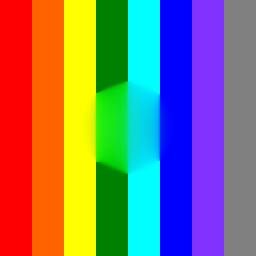
\includegraphics[width=0.8\linewidth]{images/result_ex1/fixpoint03.png}			
	\end{subfigure}
	\begin{subfigure}{0.4\linewidth}
		\centering
		
\includegraphics[width=0.8\linewidth]{images/result_ex1/fixpoint04.png}			
	\end{subfigure}
	\begin{subfigure}{0.4\linewidth}
		\centering
		
\includegraphics[width=0.8\linewidth]{images/result_ex1/fixpoint05.png}			
	\end{subfigure}
	\caption{ผลลัพธ์จากวิธีการจุดตรึง}
\end{figure}
\begin{table}[H]
	\centering
	\begin{tabular}[ht]{|c|c|c|c|c|}
		\hline
		รูปภาพ &เวลาประมวล  (วินาที) & PSNR (dB) & SSIM \\
		\hline
		1 & 24.97 & 60.95 & 1.0000 \\ 
		2 & 53.06 & 37.69 & 1.0000 \\
		3 &  190.64 & 25.17 & 0.9997 \\
		4 & 50.63  & 28.81  & 0.9999 \\
		5 & 54.74  & 40.73  & 1.0000 \\
		\hline
		เฉลี่ย & 74.81  & 38.67  & 0.9999 \\
		\hline
	\end{tabular}
	\caption{ผลลัพธ์ของวิธีจุดตรึงสำหรับการต่อเติมภาพ}
\end{table}	
\begin{figure}[H]
	\centering
	\begin{subfigure}{0.4\linewidth}
		\centering
		
\includegraphics[width=0.8\linewidth]{images/result_ex1/splitbergman01.png}
	\end{subfigure}
	\begin{subfigure}{0.4\linewidth}
		\centering
		
\includegraphics[width=0.8\linewidth]{images/result_ex1/splitbergman02.png}
	\end{subfigure}
	\begin{subfigure}{0.4\linewidth}
		\centering
		
\includegraphics[width=0.8\linewidth]{images/result_ex1/splitbergman03.png}			
	\end{subfigure}
	\begin{subfigure}{0.4\linewidth}
		\centering
		
\includegraphics[width=0.8\linewidth]{images/result_ex1/splitbergman04.png}			
	\end{subfigure}
	\begin{subfigure}{0.4\linewidth}
		\centering
		
\includegraphics[width=0.8\linewidth]{images/result_ex1/splitbergman05.png}			
	\end{subfigure}
	\caption{ผลลัพธ์จากวิธีการสปริทเบรกแมน}
\end{figure}
\begin{table}[H]
	\centering
	\begin{tabular}[ht]{|c|c|c|c|c|}
		\hline
		รูปภาพ &เวลาประมวล  (วินาที) & PSNR (dB) & SSIM \\
		\hline
		1 & 3.39 & 71.54 & 1.0000 \\ 
		2 & 10.74 & 37.08 & 1.0000 \\
		3 &  24.50 & 26.08 & 0.9997 \\
		4 & 15.80  & 29.61  & 0.9999 \\
		5 & 15.85  & 32.78  & 1.0000 \\
		\hline
		เฉลี่ย & 14.06  & 39.42  & 0.9999 \\
		\hline
	\end{tabular}
	\caption{ผลลัพธ์ของวิธีสปริทเบรกแมนสำหรับการต่อเติมภาพ}
\end{table}
	เมื่อเปรียบเทียบผลลัพธ์เฉลี่ยจากทั้ง 3 วิธีได้ดังตารางนี้ิ
	\begin{table}[H]
		\centering
		\begin{tabular}[ht]{|l|c|c|c|c|}
			\hline
			วิธีการ  & เวลาประมวล  (วินาที) & PSNR (dB) & SSIM \\
			\hline
			การเดินเวลา & 120.68 & 16.72 & 0.9960 \\
			การทำซ้ำจุดตรึง & 74.81 & 38.67 & 0.9999 \\
			การสปริทเบรกแมน & 14.06 & 39.42 & 0.9999  \\
			\hline
		\end{tabular}
		\caption{แสดงผลลัพธ์เฉลี่ยของวิธีการเชิงตัวเลขสำหรับการต่อเติมภาพ}
	\end{table}	
	\hspace{1cm} 
	ซึ่งจากทั้ง 3 วิธีที่ได้ทดสอบ จะเห็นได้ว่าวิธีการสปริทเบรกแมนใช้เวลาน้อยกว่าวิธีอื่น และมีคุณภาพ ซึ่งพิจราณาจาก ค่า PSNR และค่า SSIM มากกว่าวิธีอื่น ซึ่งผู้วิจัยจะใช้วิธีสปิทเบรกแมนมาใช้ในการพัฒนาวิธีต่อเติมภาพเป็นลำดับถัดไป
	
	\subsubsection{ขั้นตอนวิธีการสำหรับต่อเติมภาพชนิดใหม่}
	\hspace{1cm} จากวิธีการสปริทเบรกแมนนั้นจะใช้วิธีการหาคำตอบโดยวิธีการทำซ้ำจนกระทั่งลู่เข้า ทางผู้ศึกษาจึงสนใจที่หาคำตอบเริ่มต้นสำหรับการทำซ้ำที่ดีขึ้น เพื่อทำให้การทำซ้ำลู่เข้าสู่คำตอบได้เร็วขึ้น โดยการทำงานกับรูปภาพที่เล็กกว่า จากนั้นจึงทำการขยายผลลัพธ์ที่ได้ขึ้นมาทำกับภาพใหญ่ ซึ่งวิธีนี้เรียกว่าวิธีพีระมิดรูปภาพ (pyramid methods) \cite{ref:image-pyramid}  โดยผู้วิจัยจะทำการย่อขนาดรูปลงครึ่งนึงโดยใช้วิธี Bilinear Interpolation ทั้งสิ้น 4 ครั้ง จากนั้นเริ่มทำการต่อเติมภาพขนาดเล็ก จากนั้นนำผลลัพธ์ที่ได้จากภาพขนาดเล็ก ทำการขยายภาพขึ้นสองเท่าโดยใช้ Bilinear Interpolation
	 ก่อนจะนำเฉพาะส่วนที่อยู่ในโดเมนต่อเติมของภาพที่ถูกขยายมาทำการต่อเติมเพื่อให้ส่วนที่ถูกขยายขึ้นมาเป็นคำตอบเริ่มต้นสำหรับการต่อเติมภาพในชั้นถัดไป
	 	\begin{figure}[H]
	 	\centering
	 	\begin{subfigure}{0.4\linewidth}
	 		\centering
	 		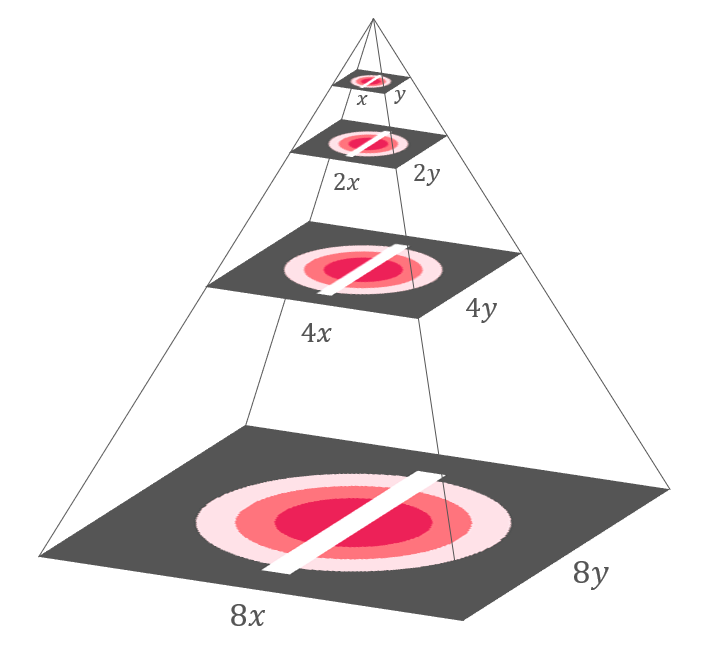
\includegraphics[width=0.8\linewidth]{images/image_inpaint_synthetic/image_pyramid.png}
	 	\end{subfigure}
 		 \caption{วิธีการพีระมิดรูปภาพ}
	 \end{figure}
 	\hspace{1cm} ซึ่งขั้นตอนวิธีสำหรับการทำพีระมิดรูปภาพสำหรับการต่อเติมภาพแบบสปริทเบรกแมนเพื่อให้ประมวลผลได้เร็วขึ้นนั้นสามารถทำได้ดังนี้
	\begin{algorithm}[H]
		\label{algo:MultiSplitBregmanColorInpaint}
		\caption{Split-bregman Color solver with Image Pyramid (Multi Resolution)}
		\KwIn{
			\\
			\hspace{1cm} $u$ is image which is damaged image \\
			\hspace{1cm} $\lambda$ is positive rational number which is regularization parameter \\
			\hspace{1cm} $\theta$ is positive rational number which is panelty parameter that shouldn't too big or too small \\
			\hspace{1cm} $N_0$ is positive interger  which is number of maximum iteration on smallest size image \\
			\hspace{1cm} $N_1$ is positive interger  which is number of maximum iteration on image that isn't the biggest neither  smallest \\
			\hspace{1cm} $N_2$ is positive interger  which is number of maximum iteration on biggest size image \\
			\hspace{1cm} $N_{gs}$ is positive integer which is number of gauss seidel iteration \\
			\hspace{1cm} $\varepsilon$ is positive rational number  which is expected relative error \\
		}
		\KwOut{inpainted image}    
		\SetKwFunction{FMain}{MultiSplitBregmanColorInpaint}
		\SetKwProg{Fn}{Function}{:}{}
		\Fn{\FMain{$u, \lambda, \theta, N_{gs}, N_0,N_1,N_2, \varepsilon,c,m$}}{
			\textbf{Initialize} $height = $ height of $u$, $width = $ width of u \\
			\If{c < m}{
				$x = BilinearResize(u,\lfloor width * 0.5 \rfloor,\lfloor height * 0.5 \rfloor)$\\
				$y = BilinearResize(\lambda,\lfloor width * 0.5 \rfloor,\lfloor height * 0.5 \rfloor)$\\
				$r = MultiSplitBregmanColorInpaint(x,y, \lambda, \theta,$ \\$ \hspace{1cm}  N_{gs}, N_0, N_1, N_2, \varepsilon,c+1,m)$\\
				$R = BilinearResize(r,width,height)$\\
				$u = CopyByDomain(u,\lambda,R)$
			}
			\uIf{$c = 1$}{$N=N_0$}
			\uElseIf{$c = m$}{$N = N_2$}
			\Else{
				$N = N_1$
			}
			$u = SplitBregmanColorInpaint(u_l, \lambda, \theta, N_{gs}, N, \varepsilon) $  \\
			\textbf{return} $u$
		}
	\end{algorithm}
	\clearpage
	โดยสำหรับขัั้นตอนวิธีนี้ จะมีขั้นตอนวิธีย่อยสำหรับช่วยอีกสองขั้นตอน คือ
	\\ 1. ขั้นตอนสำหรับการคัดลอกข้อมูลที่อยู่ในโดเมนต่อเติมจากรูป v ไปรูป u
	\begin{algorithm}[H]
		\caption{Copy image inside inpaint domain from v to u}
		\KwIn{
			\\
			\hspace{1cm} $u$ is image which is damaged image \\
			\hspace{1cm} $D$ is image which is image of inpaint domain (also compatible with regulazation paramter lambda from equation (\ref{e2}))\\
			\hspace{1cm} $v$ is image which will copy to u image
		}
		\KwOut{image}    
		\SetKwFunction{FMain}{CopyByDomain}
		\SetKwProg{Fn}{Function}{:}{}
		\Fn{\FMain{$u, D, v$}}{
			\textbf{Initialize} $height = $ height of $u$, $width = $ width of u \\
			\For{i = 0; i < height; i++}{
				\For{j = 0; j<i; j++}{
					\If{$D_{i,j} \neq 0$}{$u_{i,j} = v_{i,j}$}
				}		
			}
			\textbf{return} $ u $ 
		}	
	\end{algorithm}
 	2. ขั้นตอนสำหรับปรับขนาดภาพด้วย bilinear interpolation
	\begin{algorithm}[H]
		\caption{Bilinear Interpolation for Image resizing}
			\KwIn{
			\\
			\hspace{1cm} $u$ is image which need to resize \\
			\hspace{1cm} $x$ is positive integer which is new image height \\
			\hspace{1cm} $y$ is positive integer which  is new image width \\
		}
		\KwOut{image}
		% https://stackoverflow.com/questions/26142288
		\SetKwFunction{FMain}{BilinearResize}
		\SetKwProg{Fn}{Function}{:}{}
		\Fn{\FMain{$I,x,y$}}{
			\textbf{Initialize} $J$ is image that height $x$ and width $y$, \\ $v =$ height of $I$ and $w$ is width of $I$,\\ $S_R = \frac{c}{a}, S_C = \frac{d}{b}, r = 1,2,...,v, c = 1,2,...,w,$\\$r' = 1,2,...x, c' = 1,2,...,y,  $ \\
			$r_f = \lfloor r' \cdot S_R \rfloor $\\
			$c_f = \lfloor c' \cdot S_C \rfloor $\\
			$\triangle r = r_f - r$ \\
			$\triangle c = c_f - c$ \\
			$J(r',c') = I(r,c)\cdot(1-\triangle r)\cdot (1-\triangle c) $\\$+ I(r+1,c) \cdot \triangle r \cdot (1 - \triangle c) $\\$+I(r,c+1)\cdot(1-\triangle r)\cdot\triangle c$\\$+ I(r+1,c+1)\cdot\triangle r \cdot \triangle c$ \\
			\textbf{return} $ J $ 
		}
	\end{algorithm}
	\clearpage
	\hspace{1cm} โดยจะทำการเปรียบเทียบจำนวนครั้งในชั้นที่รูปภาพมีขนาดเล็ก จนไปถึงชั้นที่มีขนาดใหญ่ ตัวอย่าง เช่น 10/3/3/10000 หมายถึงในชั้นเล็กสุดซึ่งขนาดเป็น 32x32 พิกเซลจะทำซ้ำไม่กิน 10 ครั้ง ชั้นถัดมาขนาดเป็น 64x64 จะทำซ้ำไม่เกิน 3 ครั้ง และชั้นถัดมา ชั้นถัดมาขนาดเป็น 128x128 จะทำซ้ำ 3 ครั้ง และสุดท้ายขนาด 256x256 จะทำซ้ำไม่เกิน 10,000 ครั้งหรือจนค่าความคลาดเคลื่อนสัมพัทธ์ต่างกันไม่เกิน 0.0001 ซึ่งเมื่อทำการทดสอบแล้วได้ผลลัพธ์ดังตารางนี้
	
	\begin{table}[H]
		\footnotesize
		\centering
		\begin{tabular}[ht]{|l|c|c|c|c|c|}
			\hline
			รูปแบบการทำซ้ำ  & รูปภาพ &เวลาประมวล  (วินาที) & PSNR (dB) & SSIM \\
			\hline
			ไม่ใช้พีระมิดรูปภาพ & 1 & 4.49  & 71.54 & 1.0000 \\ 
			& 2 & 13.16 & 37.08 & 1.0000 \\
			& 3 & 29.46 & 26.08 & 0.9997 \\
			& 4 & 20.50 & 29.61 & 0.9999 \\
			& 5 & 19.32 & 32.78 & 1.0000 \\
			\hline
			10/1/1/10000 & 1 & 2.44 & 69.59& 1.0000 \\
			& 2 & 11.31 &37.04 & 1.0000 \\
			& 3 & 23.48 & 27.34 & 0.9998 \\
			& 4 & 16.60 & 29.42 & 0.9999 \\
			& 5 & 13.75 & 33.53 & 1.0000 \\
			\hline
			10/3/3/10000  & 1 & 2.24 & 69.96 & 1.0000\\
			& 2 & 10.91 & 37.05 & 1.0000 \\
			& 3 & 21.99 & 27.66 & 0.9998 \\
			& 4 & 12.70 & 29.35 & 0.9999 \\
			& 5 & 11.49 & 33.69 & 1.0000\\
			\hline
			10/10/10/10000  & 1 & 1.83 & 71.58 & 1.0000 \\
			& 2 & 7.83 & 37.05 & 1.0000 \\
			& 3 & 16.75 & 28.62 & 0.9998 \\
			& 4 & 11.89 & 29.32 & 0.9999 \\
			& 5 & 8.00 & 34.26 & 1.0000 \\
			\hline
			100/1/1/10000  & 1 & 1.43 & 67.63 & 1.0000\\
			& 2 & 7.17 & 37.10 & 1.0000 \\
			& 3 & 20.86 & 27.70 & 0.9998 \\
			& 4 & 12.80 & 29.64 & 0.9999\\
			& 5 & 9.17 & 33.14 & 1.0000 \\
			\hline
			100/3/3/10000  & 1 & 1.68 & 71.18 & 1.0000 \\
			& 2 & 7.41 & 37.11 & 1.0000\\
			& 3 & 21.08 & 28.00 & 0.9998 \\
			& 4 & 13.28 & 29.38 & 0.9999 \\
			& 5 & 7.96 & 33.34 & 1.0000\\
			\hline
			100/10/10/10000  & 1 & 1.76 & 71.56 & 1.0000 \\
			& 2 & 7.32 & 37.04 & 1.0000\\
			& 3 & 16.62 & 28.65 & 0.9998 \\
			& 4 & 13.18 & 29.39 & 0.9999\\
			& 5 & 7.45 & 33.94 & 1.0000 \\
			\hline
		\end{tabular}
		\caption{แสดงผลลัพธ์ของการใช้พีระมิดภาพในการต่อเติมในชั้นที่ต่างกัน}
\end{table}	
	\begin{table}[H]
		\centering
		\begin{tabular}[ht]{|l|c|c|c|c|}
			\hline
			รูปแบบการทำซ้ำ  & เวลาประมวล  (วินาที) & PSNR (dB) & SSIM \\
			\hline
			ไม่ใช้พีระมิดรูปภาพ & 17.38 & 39.42 & 0.9999 \\
			10/1/1/10000 & 13.52 & 39.38 & 0.9999 \\
			10/3/3/10000 & 11.86 & 39.54 & 0.9999 \\
			10/10/10/10000 & 9.26 & 40.17 & 0.9999\\
			100/1/1/10000 & 10.28 & 39.04 & 0.9999\\
			100/3/3/10000 & 10.28 & 39.80 & 0.9999\\
			100/10/10/10000 & 9.27 & 40.12 & 0.9999 \\
			\hline
		\end{tabular}
		\caption{แสดงผลลัพธ์เฉลี่ยของการใช้พีระมิดภาพในการต่อเติมในชั้นที่ต่างกัน}
	\end{table}	
	
	\hspace{1cm}จากตารางจะสังเกตว่า ยิ่งจำนวนการทำซ้ำในชั้นที่รูปภาพมีขนาดเล็กจำนวนมากครั้ง จะยิ่งทำให้เวลาประมวลผลที่ใช้ในการต่อเติมภาพ ใช้เวลาน้อยลง
	
	\hspace{1cm} ซึ่งนอกจากนี้แล้ว ผู้วิจัยยังได้สังเกตอีกว่า การทำซ้ำนั้น จะลู่เข้าเร็วในช่วงแรก จากนั้นความเร็วในการลู่เข้าจะลดลง ซึ่งทำให้การทำซ้ำเพียงไม่กี่ครั้งในรูปภาพขนาดใหญ่สุด มีผลลัพธ์ใกล้เคียงกับภาพต้นฉบับได้
	
	\begin{figure}[H]
		\centering
		\begin{subfigure}{0.4\linewidth}
			\centering
			
\includegraphics[width=0.8\linewidth]{images/just10enough/only10time.png}
			\caption{ชั้นใหญ่สุด 10 ครั้ง}
		\end{subfigure}
		\begin{subfigure}{0.4\linewidth}
			\centering
			
\includegraphics[width=0.8\linewidth]{images/just10enough/only100time.png}
			\caption{ชั้นใหญ่สุด 100 ครั้ง}
		\end{subfigure}
		\begin{subfigure}{0.4\linewidth}
			\centering
			
\includegraphics[width=0.8\linewidth]{images/just10enough/only1000time.png}			
			\caption{ชั้นใหญ่สุด 1,000 ครั้ง}
		\end{subfigure}
		\begin{subfigure}{0.4\linewidth}
			\centering
			
\includegraphics[width=0.8\linewidth]{images/just10enough/only10000time.png}			
			\caption{ชั้นใหญ่สุด 10,000 ครั้ง}
		\end{subfigure}
		\caption{พีระมิดที่ลำดับการทำซ้ำเป็น 10/10/10 และชั้นใหญ่สุดทำในจำนวนครั้งที่ต่างกัน}
	\end{figure}
	
	 โดยผู้วิจัยจึงกำหนดให้การทำซ้ำในรูปภาพขนาดใหญ่สุดมีการทำซ้ำเพียง 10 ครั้ง และพบว่าได้ผลลัพธ์ดังนี้
		\begin{table}[H]
		\centering
		\small
		\begin{tabular}[ht]{|l|c|c|c|c|c|}
			\hline
			รูปแบบการทำซ้ำ  & รูปภาพ &เวลาประมวล  (วินาที) & PSNR (dB) & SSIM \\
			\hline
			ไม่ใช้พีระมิดรูปภาพ & 1 & 0.30  & 26.71  & 0.9998 \\ 
			& 2 & 0.39  & 18.39  & 0.9982 \\
			& 3 & 0.38 & 13.66  & 0.9944 \\
			& 4 & 0.40  & 12.86 & 0.9934 \\
			& 5 & 0.38 & 14.69 &  0.9956\\
			\hline
			10/1/1/10 & 1 & 0.29 & 40.10 & 1.0000\\
			& 2 & 0.41 & 31.28 & 0.9999 \\
			& 3 & 0.46 & 16.51 & 0.9970 \\
			& 4 & 0.47 & 26.56 & 0.9998\\
			& 5 & 0.39 & 28.25 & 0.9998 \\
			\hline
			10/3/3/10  & 1 & 0.28 & 42.53 & 1.0000\\
			& 2 & 0.36 & 32.91 & 1.0000 \\
			& 3 & 0.35 & 16.88 & 0.9972 \\
			& 4 & 0.34 & 27.06 &  0.9998 \\
			& 5 & 0.34 & 29.76 & 0.9999 \\
			\hline
			10/10/10/10  & 1 & 0.31 & 50.06 & 1.0000 \\
			& 2 & 0.41 & 34.01 & 1.0000\\
			& 3 & 0.38 & 18.19 & 0.9980\\
			& 4 & 0.39 & 27.50 & 0.9998\\
			& 5 & 0.40 & 33.05 &  1.0000\\
			\hline
			100/1/1/10  & 1 & 0.27 & 43.97 & 1.0000 \\
			& 2 & 0.37  & 31.28 & 0.9999\\
			& 3 & 0.36 & 24.98 & 0.9997\\
			& 4 & 0.36  &28.05 & 0.9998\\
			& 5 & 0.36 & 29.24 & 0.9999 \\
			\hline
			100/3/3/10  & 1 & 0.29 & 45.08& 1.0000 \\
			& 2 & 0.36 & 32.36 & 0.9999\\
			& 3 & 0.40 & 0.40 & 0.9996\\
			& 4 & 0.38 & 27.88 & 0.9998\\
			& 5 & 0.37 & 30.28 & 0.9999 \\
			\hline
			100/10/10/10  & 1 & 0.28 & 50.05 &  1.0000\\
			& 2 & 0.41 & 33.25 &  1.0000\\
			& 3 & 0.42 & 23.51 & 0.9995 \\
			& 4 & 0.42 & 27.78 & 0.9998 \\
			& 5 & 0.39 & 32.38 & 0.9999 \\
			\hline
		\end{tabular}
		\caption{แสดงผลลัพธ์ของการใช้พีระมิดภาพในการต่อเติมโดยกำหนดให้ชั้นรูปภาพขนาดใหญ่สุดทำซ้ำเพียง 10 ครั้ง}
	\end{table}	
	\begin{table}[H]
		\centering
		\begin{tabular}[ht]{|l|c|c|c|c|}
			\hline
			รูปแบบการทำซ้ำ  & เวลาประมวล  (วินาที) & PSNR (dB) & SSIM \\
			\hline
			ไม่ใช้พีระมิดรูปภาพ & 0.37 & 17.26 & 0.9963  \\
			10/1/1/10 & 0.40 & 28.54 & 0.9993 \\
			10/3/3/10 & 0.33 & 29.83  & 0.9994 \\
			10/10/10/10 & 0.38 & 32.56 & 0.9995 \\
			100/1/1/10 & 0.34 & 31.50 & 0.9999 \\
			100/3/3/10 & 0.36 & 27.20 & 0.9999 \\
			100/10/10/10 & 0.38 & 33.39 & 0.9998 \\
			\hline
		\end{tabular}
		\caption{แสดงผลลัพธ์เฉลี่ยของการใช้พีระมิดภาพในการต่อเติมโดยกำหนดให้ชั้นรูปภาพขนาดใหญ่สุดทำซ้ำเพียง 10 ครั้ง}
	\end{table}	

	\hspace{1cm}จากตารางจะเห็นว่า การทำซ้ำในชั้นที่รูปภาพมีขนาดเล็กมากจำนวนมาก ไม่ช่วยให้การประมวลผลได้เร็วขึ้น ผู้วิจัยจึงเลือกใช้การทำซ้ำแบบ 10/3/3/10 ในการต่อเติมภาพ
	
	\subsubsection{การทดสอบประสิทธิภาพในการซ่อมแซมภาพจิตรกรรมไทยโบราณ}
	\hspace{1cm}ซึ่งภาพจิตรกรรมทีี่ใช้ทดสอบ มีทั้งสิ้น 5  ภาพ โดยแต่ละภาพเป็นภาพสีที่มีขนาด 256x256 พิกเซล ซึ่งทั้ง 5 ภาพได้แก่ ภาพที่ \ref{image:thaiart_case01_original} \footnote{ภาพถ่ายที่วัดแก้วไพฑูรย์; ภาพจาก  https://commons.wikimedia.org/wiki/File:จิตรกรรมฝาผนัง\_วัดแก้วไพฑูรย์\_(7).jpg สืบค้นเมื่อวันที่ 23 กันยายน 2561}   และภาพที่ \ref{image:thaiart_case02_original} \footnote{ภาพถ่ายที่วัดแก้วไพฑูรย์; ภาพจาก  https://commons.wikimedia.org/wiki/File:จิตรกรรมฝาผนัง\_วัดแก้วไพฑูรย์\_(2).jpg สืบค้นเมื่อวันที่ 23 กันยายน 2561} คือ จิตรกรรมฝาผนังวัดแก้วไพฑูรย์ ภาพที่ \ref{image:thaiart_case03_original} \footnote{ภาพถ่ายที่วัดพระยืนพุทธบาทยุคล; ภาพจาก https://commons.wikimedia.org/wiki/File:Wat\_Phra\_Yuen \_Phutthabat\_Yukhon\_01.jpg สืบค้นเมื่อวันที่ 23 กันยายน 2561}  คือ จิตรกรรมฝาผนังวัดพระยืนพุทธบาทยุคล ภาพที่ \ref{image:thaiart_case04_original} \footnote{ภาพถ่ายที่วัดคงคาราม; ภาพจาก  https://commons.wikimedia.org/wiki/File:จิตรกรรม\_อุโบสถวัดคงคาราม.JPG สืบค้นเมื่อวันที่ 23 กันยายน 2561} คือ จิตรกรรมฝาผนังวัดคงคาราม และภาพที่ \ref{image:thaiart_case05_original} \footnote{ภาพถ่ายที่วัดท่าถนน; ภาพจาก  https://commons.wikimedia.org/wiki/File:Wat\_Tha\_Thanon\_05.JPG สืบค้นเมื่อวันที่ 23 กันยายน 2561} คือ จิตรกรรมฝาผนังวัดท่าถนน
	โดยจะทำให้ข้อมูลข้องทั้ง 5 ภาพเกิดความเสียหาย โดยใช้รอยความเสียหายจากภาพพระเจ้าสร้างอดัม
	
	\begin{figure}[H]
		\centering
		\begin{subfigure}{0.4\linewidth}
			\centering
			
\includegraphics[width=0.8\linewidth]{images/thaiart/case01-original.png}
			\caption{วัดแก้วไพฑูรย์}
			\label{image:thaiart_case01_original}
		\end{subfigure}
		\begin{subfigure}{0.4\linewidth}
			\centering
			
\includegraphics[width=0.8\linewidth]{images/thaiart/case02-original.png}
			\caption{วัดแก้วไพฑูรย์}
			\label{image:thaiart_case02_original}
		\end{subfigure}
		\begin{subfigure}{0.4\linewidth}
			\centering
			
\includegraphics[width=0.8\linewidth]{images/thaiart/case03-original.png}
			\caption{วัดพระยืนพุทธบาทยุคล}
			\label{image:thaiart_case03_original}			
		\end{subfigure}		
		\begin{subfigure}{0.4\linewidth}
			\centering
			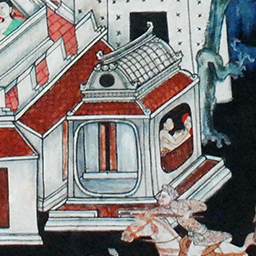
\includegraphics[width=0.8\linewidth]{images/thaiart/case04-original.png}
			\caption{วัดคงคาราม}
			\label{image:thaiart_case04_original}			
		\end{subfigure}
		\begin{subfigure}{0.4\linewidth}
			\centering
			
\includegraphics[width=0.8\linewidth]{images/thaiart/case05-original.png}
			\caption{วัดท่าถนน}
			\label{image:thaiart_case05_original}			
		\end{subfigure}
		\begin{subfigure}{0.4\linewidth}
			\centering
			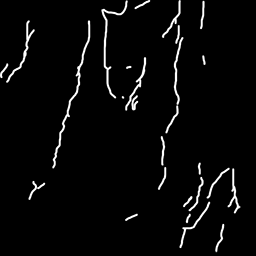
\includegraphics[width=0.8\linewidth]{images/thaiart/inpaint-domain.png}
			\caption{รอยความเสียหาย}
		\end{subfigure}
		\caption{ภาพต้นฉบับสำหรับใช้ในการทดสอบ}
	\end{figure}
	\begin{figure}[H]
	\centering
	\begin{subfigure}{0.4\linewidth}
		\centering
		
\includegraphics[width=0.8\linewidth]{images/thaiart/case01-toinpaint.png}
	\end{subfigure}
	\begin{subfigure}{0.4\linewidth}
		\centering
		
\includegraphics[width=0.8\linewidth]{images/thaiart/case02-toinpaint.png}
	\end{subfigure}
	\vspace{1cm}
	\begin{subfigure}{0.4\linewidth}
		\centering
		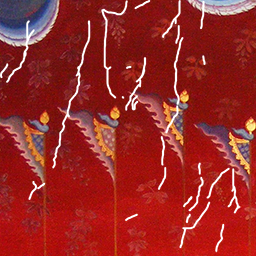
\includegraphics[width=0.8\linewidth]{images/thaiart/case03-toinpaint.png}			
	\end{subfigure}
	\begin{subfigure}{0.4\linewidth}
		\centering
		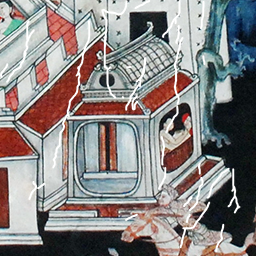
\includegraphics[width=0.8\linewidth]{images/thaiart/case04-toinpaint.png}			
	\end{subfigure}
	\begin{subfigure}{0.4\linewidth}
		\centering
		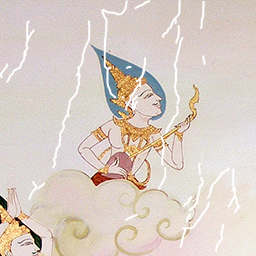
\includegraphics[width=0.8\linewidth]{images/thaiart/case05-toinpaint.png}			
	\end{subfigure}
	\caption{ภาพที่ทำให้เสียหาย}
\end{figure}
	 \hspace{1cm} จากนั้นทำการทดสอบการต่อเติมภาพทั้ง 5 โดยทดสอบวิธีสปริทเบรกแมน และวิธีทีที่พัฒนาขึ้นโดยใช้วิธีการสปริทเบรกแมนพร้อมทั้งการใช้พีระมิดรูปภาพที่มีการทำซ้ำแต่ละชั้นเป็น 10/3/3/10  ได้ผลลัพธ์ออกมาเป็นดังนี้
	\begin{figure}[H]
		\centering
		\begin{subfigure}{0.4\linewidth}
			\centering
			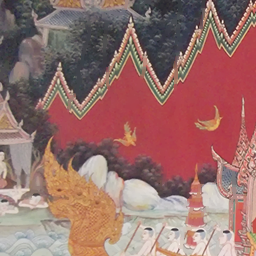
\includegraphics[width=0.8\linewidth]{images/result_ex4/splitbergman_case01.png}
		\end{subfigure}
		\begin{subfigure}{0.4\linewidth}
			\centering
			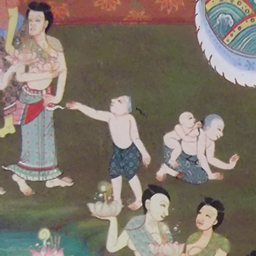
\includegraphics[width=0.8\linewidth]{images/result_ex4/splitbergman_case02.png}
		\end{subfigure}
		\begin{subfigure}{0.4\linewidth}
			\centering
			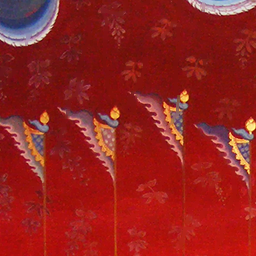
\includegraphics[width=0.8\linewidth]{images/result_ex4/splitbergman_case03.png}			
		\end{subfigure}
		\begin{subfigure}{0.4\linewidth}
			\centering
			\includegraphics[width=0.8\linewidth]{images/result_ex4/splitbergman_case04.png}			
		\end{subfigure}
		\begin{subfigure}{0.4\linewidth}
			\centering
			\includegraphics[width=0.8\linewidth]{images/result_ex4/splitbergman_case05.png}			
		\end{subfigure}
		\caption{ผลลัพธ์จากวิธีการสปริทเบรกแมน}
	\end{figure}
	\begin{table}[H]
		\centering
		\begin{tabular}[ht]{|c|c|c|c|c|}
			\hline
			รูปภาพ &เวลาประมวล  (วินาที) & PSNR (dB) & SSIM \\
			\hline
			1 & 2.95 & 33.92 & 1.0000 \\ 
			2 & 2.64 & 37.33 & 1.0000 \\
			3 &  3.49 & 37.21 & 1.0000 \\
			4 & 2.70  & 29.47  & 1.0000 \\
			5 & 15.85  & 32.78  & 1.0000 \\
			\hline
			เฉลี่ย & 2.72  & 34.89  & 1.0000 \\
			\hline
		\end{tabular}
		\caption{ผลลัพธ์การซ่อมแซมภาพศิลปะไทยจากวิธีการสปิทเบรกแมน}
	\end{table}
	\begin{figure}[H]
		\centering
		\begin{subfigure}{0.4\linewidth}
			\centering
			\includegraphics[width=0.8\linewidth]{images/result_ex4/multisplitbergman_case01.png}
		\end{subfigure}
		\begin{subfigure}{0.4\linewidth}
			\centering
			\includegraphics[width=0.8\linewidth]{images/result_ex4/multisplitbergman_case02.png}
		\end{subfigure}
		\begin{subfigure}{0.4\linewidth}
			\centering
			\includegraphics[width=0.8\linewidth]{images/result_ex4/multisplitbergman_case03.png}			
		\end{subfigure}
		\begin{subfigure}{0.4\linewidth}
			\centering
			\includegraphics[width=0.8\linewidth]{images/result_ex4/multisplitbergman_case04.png}			
		\end{subfigure}
		\begin{subfigure}{0.4\linewidth}
			\centering
			\includegraphics[width=0.8\linewidth]{images/result_ex4/multisplitbergman_case05.png}			
		\end{subfigure}
		\caption{ผลลัพธ์จากวิธีการที่พัฒนาขึ้น}
	\end{figure}
		\begin{table}[H]
		\centering
		\begin{tabular}[ht]{|c|c|c|c|c|}
			\hline
			รูปภาพ &เวลาประมวล  (วินาที) & PSNR (dB) & SSIM \\
			\hline
			1 & 0.40 & 34.13 & 1.0000 \\ 
			2 & 0.40 & 38.18 & 1.0000 \\
			3 &  0.39 & 37.73 & 1.0000 \\
			4 & 0.38  & 29.38  & 1.0000 \\
			5 & 0.39  & 37.11  & 1.0000 \\
			\hline
			เฉลี่ย & 0.39  & 35.30  & 1.0000 \\
			\hline
		\end{tabular}
		\caption{ผลลัพธ์การซ่อมแซมภาพศิลปะไทยจากวิธีที่พัฒนาขึ้น}
	\end{table}	 
	\hspace{1cm}ซึ่งทั้งสองวิธี ได้ผลลัพธ์การซ่อมแซมศิลปะไทยเฉลี่ยออกมาดังนี้
	\begin{table}[H]
		\centering
		\begin{tabular}[ht]{|l|c|c|c|c|}
			\hline
			วิธีการ  & เวลาประมวล  (วินาที) & PSNR (dB) & SSIM \\
			\hline
			สปริทเบรกแมน & 2.72 & 34.89 & 1.0000 \\ 
			วิธีการที่พัฒนาขึ้น & 0.39 & 35.30 & 1.0000 \\
			\hline
		\end{tabular}
		\caption{แสดงผลลัพธ์เฉลี่ยของการซ่อมแซมภาพศิลปะไทย}
	\end{table}	
	\hspace{1cm} จากตารางจะเห็นได้ว่า วิธีที่พัฒนาขึ้นนั้นสามารถทำงานได้เร็วกว่าวิธีสปริทเบรกแมนเดิม และยังมีคุณภาพที่ดีขึ้นด้วย
	
	
	
	\subsection{การลบบทบรรยายบนอนิเมะ}
	\hspace{1cm} สำหรับการลบบทบรรยายอนิเมะ จะใช้วิดีโอ Anime Festival Asia Special Video - feat. Inori Aizawa ซึ่งผลิตโดย Collateral Damage Studios โดยจะตัดวิดีโอ 1 นาทีแรกสำหรับการทดลอง โดยวิดีโอดังกล่าวขนาด 1280 x 720 พิกเซล แต่เนื่องจากโดยปกติแล้ว อนิเมะมักมีบรรทัดเพียง 1 ถึง 2 บรรทัด จึงทำการแบ่งวิดีโอออกอีกเป็น 5 ส่วนได้ขนาดเป็น 1280 x 144 พิกเซลก่อนนำไปทดสอบในลำดับถัดไป
	\hspace{1cm} และสำหรับบทบรรยายที่จะใช้ทดสอบนั้น เนื่องจากวิดีโอ Anime Festival Asia Special Video - feat. Inori Aizawa ไม่มีคำพูดใดๆ จึงใช้บทความ lorem ipsum เป็นบทบรรยาย โดยจะทำการแสดงบทบรรยาย 1 บรรทัด ความยาว 3 วินาที ทุก 2 วินาที นั่นคือในวิดีโอดังกล่าวจะมีบทบรรยายทั้งสิ้น 20 บรรทัด	
	
	\begin{figure}[H]
		\centering
		\begin{subfigure}{0.8\linewidth}
			\centering
			\includegraphics[width=0.8\linewidth]{images/inori-subbed-preview.png}
		\end{subfigure}
		\caption{การแบ่งไฟล์วิดีโอเป็น 5 ส่วนสำหรับใช้เป็น 5 ชุดทดสอบ}
	\end{figure}
	
	\hspace{1cm}เนื่องจากไฟล์วิดีโอนั้นประกอบชุดของภาพหลายภาพ ทำให้ขั้นตอนวิธีการลบคำบรรยายออกจากวิดีโอ จะต้องทำการต่อเติมบริเวณที่เป็นบทบรรยายทีละภาพ นั่นคือจะมีขั้นตอนวิธีดังนี้ \\
	
	\begin{algorithm}[H]
		\caption{remove subtitle from video}
		\KwIn{
			 $V$ is video with subtitle \\
		}
		\KwOut{video without subtitle}
		\SetKwFunction{FMain}{RemoveSubtitle}
		\SetKwProg{Fn}{Function}{:}{}
		\Fn{\FMain{$V$}}{
			\ForEach{$u_i$ is frame number $i$ of video $V$}{
				$\bullet$ find inpaint domain $D$ from $u_i$\\
				$\bullet$ inpaint image $u_i$ by using domain $D$\\
			}
			\textbf{return} $ V $ 
		}
	\end{algorithm}
	\vspace{1cm}
	\hspace{1cm} โดยขั้นตอนการต่อเติมภาพ $u_i$ ด้วยโดเมนต่อเติม $D$ นั้นจะสามารถใช้วิธีการเดียวกับการซ่อมแซมภาพศิลปะไทยได้ ส่วนการหาบทบรรยายอนิเมะ จะกล่าวถึงในขั้นถัดไป
	
	
	\subsubsection{การหาบทบรรยายบนอนิเมะ}	
	\hspace{1cm}ก่อนจะลบบทบรรยายนั้น จำเป็นต้องหาบทบรรยายในภาพให้ได้เสียก่อน โดยบทบรรยายของอนิเมะนั้น มักจะใช้ขอบของตัวอักษรเป็นสีดำ อีกทั้งบทบรรยายนั้นจะลอยห่างออกมาจากขอบของวิดีโอ และขนาดของคำบรรยายนั้นจะมีขนาดอยู่ประมาณหนึ่งไม่ใหญ่หรือไม่เล็กเกินไป ด้วยสมบัตินี้เองทำให้จึงสามารถหาบริเวณบนเฟรมที่เป็นบทบรรยายได้โดยจะมีวิธีหาพื้นที่ซึ่งเป็นบทบรรยายดังนี้
	
	\vspace{1cm}
	
	\begin{algorithm}[H]
		\caption{finding subtitle}
		\KwIn{
			\\
			\hspace{1cm} $u$ is image which is part of anime frame\\
		}
		\KwOut{inpainting domain (subtitle)}    
		\SetKwFunction{FMain}{FindSubtitle}
		\SetKwProg{Fn}{Function}{:}{}
		\Fn{\FMain{$u$}}{
			$\bullet$  to find the edge of subtitle. we find color black in image $u$ by mark black color region as white and otherwise color is mark to black.\\
			$\bullet$ change white region in image to black and black region in image to white. now we get white region in image \\
			$\bullet$ remove any white region that attach to edge of image, because subtitle always floating away  from screen edge.\\
			$\bullet$  remove white region that too big to be subtitle \\
			$\bullet$  remove white region that too small to be subtitle \\
			$\bullet$ dilate white region with subtitle edge width \\
			$\bullet$ every white region left on image should be subtitle.
		}	
	\end{algorithm}
	\clearpage
	\hspace{1cm} ซึ่งวิธีการหาบทบรรยายที่กล่าวไปข้างต้น จะทำการทดสอบกับบทความ lorem ipsum ที่ถูกแปลเป็นภาษาไทย ภาษาอังกฤษ และภาษาญี่ปุ่น โดยมีความสามารถในการหาโดเมนต่อเติมใบบทบรรยายภาษาต่างๆ ดังนี้
	%TODO ทำภาพแถวละ2
	\begin{table}[H]
		\centering
		\begin{tabular}[ht]{|l|c|c|c|c|c|}
			\hline
			ภาษา  & วีดีโอ & จำนวนพิกเซลในโดเมน & จำนวนพิกเซลที่ตรวจพบ & จำนวนพิกเซลที่ผิดพลาด & ร้อยละการผิดพลาด \\
			\hline
			ไทย & 1 & 23,190,522  & 24,044,004 & 2,108,772 &9.09\\
				 & 2 & 23,232,287 & 24,026,820 & 2,204,025 & 9.49\\
				& 3 & 23,189,082 & 24,300,589 & 2,081,340 & 8.98\\
				& 4 & 23,277,706 & 23,796,276  & 2,126,004 & 9.13\\
				& 5 & 23,221,502 & 24,247,935 & 2,185,864 & 9.41\\
			\hline
			อังกฤษ & 1 & 27,281,185 & 28,631,063 & 3,477,960  & 12.75\\
			& 2 & 27,269,671 & 28,513,248 & 3,514,859 & 12.89\\
			& 3 & 27,325,148 & 28,611,300 & 3,815,082 & 13.96\\
			& 4 & 27,191,136 & 28,527,105 & 3,854,121 & 14.17\\
			& 5 & 27,326,584 & 28,709,405 & 3,909,582 & 14.31\\
			\hline
			ญี่ปุ่น & 1 & 28,509,908 & 30,058,101 &  3,953,067 & 13.87\\
			& 2 & 28,534,363  & 30,023,923 & 3,565,609 & 12.50\\
			& 3 & 28,537,968 & 30,015,047 & 3,553,128 & 12.45\\
			& 4 & 28,579,778 & 30,065,985 & 3,961,319 & 13.86\\
			& 5 & 28,558,848 & 30,354,275 & 3,671,730 & 12.86\\
			\hline
		\end{tabular}
		\caption{แสดงความคาดเคลื่อนของการหาโดเมนต่อเติม ในบทบรรยายภาษาต่างๆ}
	\end{table}
	\begin{table}[H]
		\centering
		\begin{tabular}[ht]{|l|c|c|c|c|}
			\hline
			ภาษา  & จำนวนพิกเซลในโดเมน & จำนวนพิกเซลที่ตรวจพบ & จำนวนพิกเซลที่ผิดพลาด & ร้อยละการผิดพลาด \\
			\hline
			ไทย & 23,222,220 & 24,083,125 & 2,141,201 & 9.22 \\
			อังกฤษ & 27,278,745 & 28,598,424 & 3,714,321 & 13.62 \\
			ญี่ปุ่น & 28,544,173 & 30,103,466 & 3,740,971 & 13.11 \\
			\hline
		\end{tabular}
		\caption{แสดงความคาดเคลื่อนเฉลี่ยของการหาโดเมนต่อเติม ในบทบรรยายภาษาต่างๆ}
	\end{table}	
	
	\hspace{1cm} จากการทดลองทั้ง  3 ภาษาพบว่าวิธีการหาคำบรรยายนี้ มีร้อยละการผิดพลาดเฉลี่ยอยู่ที่ 11.98 ซึ่งการทดลองจากนี้ไปจะใช้วิธีการหาคำบรรยายนี้ในการหาโดเมนต่อเติมแบบอัตโนมัติ
	
	\subsubsection{การลบคำบรรยายจากบทอนิเมะ}
	\hspace{1cm} สำหรับอนิเมะนั้น แต่ละเฟรมจะเป็นรูปภาพ เราจึงสามารถประยุกต์ใช้วิธีการซ่อมแซมภาพจิตรกรรมไทย มาใช้ในการลบคำบรรยายได้ แต่ผู้วิจัยก็ได้สังเกตว่า สำหรับอนิเมะที่เป็นวิดีโอแล้ว ในขณะที่ประมวลผลวิดีโอ เราสามารถใช้ผลการต่อเติมภาพจากภาพที่แล้ว มาใช้เป็นคำตอบเริ่มต้นจึงได้ว่าขึ้นตอนการลบบทบรรยายออกจากวิดีโอมีดังนี้\\
	\begin{algorithm}[H]
		\caption{subtitle remove with reference from previous frame}
		\KwIn{$V$ is video with subtitle}
		\KwOut{video without frame}    
		\SetKwFunction{FMain}{RemoveSubitlte}
		\SetKwProg{Fn}{Function}{:}{}
		\Fn{\FMain{$V$}}{
			\textbf{initialize} $i =1$, $N_{f}$ is total frame in $V$ \\
			\While{$i < N_f - 1$}{
				$u_i$ is frame number $i$ of video $V$ \\
				$u_{i+1}$ is frame number $i$ of video $V$ \\
				$D$ is inpainted domain of subtitle from frame $u_{i+1}$ \\
				$u_{i+1} = BorrowFrame(u_{i},D,u_{i+1})$
			}
			\textbf{return} $V$
		}	
	\end{algorithm}
	\vspace{1cm}
	\hspace{1cm} โดย $BorrowFrame(u_{i},D,u_{i+1})$  คือขั้นตอนวิธีที่ \ref{algo:borrowframe} ซึ่งในทำนองเดียวกันเราสามารถเปลี่ยน $BorrowFrame(u_{i},D,u_{i+1})$ เป็น $SkipFrame(u_{i},D,u_{i+1})$ เพื่อใช้กับขั้นตอนวิธี \ref{algo:skipframe} และเปลี่ยนเป็น  $SkipฺBorrowFrame(u_{i},D,u_{i+1})$ เพื่อใช้กับขั้นตอนวิธี \ref{algo:skipnborrowframe} ได้
	\vspace{1cm}
	ขั้นตอนวิธี การยืมเฟรม จะเป็นการนำผลลัพธ์จากเฟรมก่อนหน้ามาเป็นคำตอบในการเริ่มต้นในการประมวลผลเพื่อให้ผลลัพธ์ลู่เข้าได้เร็วขึ้น
	\begin{algorithm}[H]
		\label{algo:borrowframe}
		\caption{ฺBorrow Frame Technique}
		\KwIn{
			\\
			\hspace{1cm} $u$ is image which is current frame\\
			\hspace{1cm} $v$ is image which is previous frame\\
			\hspace{1cm} $D$ is image which is image of inpaint domain \\
		}
		\KwOut{inpainted frame}    
		\SetKwFunction{FMain}{BorrowFrame}
		\SetKwProg{Fn}{Function}{:}{}
		\Fn{\FMain{$u, D, v$}}{
			$U = CopyByDomain(u,D,\vec{0})$ \\
			$V = CopyByDomain(v,D,\vec{0})$ \\
			$s =$ SSIM of $U$ and $V$ \\
			\If{s > 0.9}{
				$u = CopyByDomain(u,D,v)$
			}
			\textbf{return} $MultiSplitBregmanColorInpaint(u,D,\lambda, \theta, g, N_0, N_1, N_2, \varepsilon,1,m)$
		}	
	\end{algorithm}
	\clearpage
	ขั้นตอนวิธี การข้ามเฟรม สำหรับเฟรมใดที่ผลลัพธ์ใกล้เคียงกันมาก จะทำการข้ามการต่อเติมภาพในเฟรมนั้นไปโดยใช้คำตอบจากเฟรมก่อนหน้าแทนเพื่อลดเวลาการประมวลผล
	\begin{algorithm}[H]
		\label{algo:skipframe}
		\caption{skip frame technique}
		\KwIn{
			\\
			\hspace{1cm} $u$ is image which is current frame\\
			\hspace{1cm} $v$ is image which is previous frame\\
			\hspace{1cm} $D$ is image which is image of inpaint domain \\
		}
		\KwOut{inpainted frame}    
		\SetKwFunction{FMain}{SkipFrame}
		\SetKwProg{Fn}{Function}{:}{}
		\Fn{\FMain{$u, D, v$}}{
			$U = CopyByDomain(u,D,\vec{0})$ \\
			$V = CopyByDomain(v,D,\vec{0})$ \\
			$s =$ SSIM of $U$ and $V$ \\
			\If{s > 0.95}{
				\textbf{return} $CopyByDomain(u,D,v)$ 
			}
			\textbf{return} $MultiSplitBregmanColorInpaint(u,D,\lambda, \theta, g, N_0, N_1, N_2, \varepsilon,1,m)$
		}	
	\end{algorithm}
	\vspace{1cm}
	ขั้นตอนวิธี การข้ามและยืมเฟรม คือขั้นตอนวิธี \ref{algo:borrowframe} และขั้นตอนวิธี \ref{algo:skipframe} ที่นำมาประยุกต์ใช้งานร่วมกัน
	\begin{algorithm}[H]
		\label{algo:skipnborrowframe}
		\caption{Skip and borrow frame technique}
		\KwIn{
			\\
			\hspace{1cm} $u$ is image which is current frame\\
			\hspace{1cm} $v$ is image which is previous frame\\
			\hspace{1cm} $D$ is image which is image of inpaint domain \\
		}
		\KwOut{inpainted frame}    
		\SetKwFunction{FMain}{SkipBorrowFrame}
		\SetKwProg{Fn}{Function}{:}{}
		\Fn{\FMain{$u, D, v$}}{
			$U = CopyByDomain(u,D,\vec{0})$ \\
			$V = CopyByDomain(v,D,\vec{0})$ \\
			$s =$ SSIM of $U$ and $V$ \\
			\uIf{s > 0.95}{
				\textbf{return} $CopyByDomain(u,D,v)$ 
			}
			\ElseIf{s > 0.9}{
				$u = CopyByDomain(u,D,v)$ 
			}
			\textbf{return} $MultiSplitBregmanColorInpaint(u,D,\lambda, \theta, g, N_0, N_1, N_2, \varepsilon,1,m)$
		}	
	\end{algorithm}
	
	\clearpage
	 ซึ่งผลลัพธ์เปรียบเทียบระหว่างแบบใช้วิธี ยืมเฟรม ใช้วิธีข้ามเฟรม และวิธีข้ามและยืมเฟรม ได้ผลดังตาราง
		\begin{table}[H]
		\centering
		\begin{tabular}[ht]{|l|c|c|c|c|c|}
			\hline
			วิธีการ  & วิดีโอ &เวลาประมวล  (วินาที) & PSNR (dB) & SSIM \\
			\hline
			สปริทเบรกแมน & 1 & 130.03  & 32.19 & 0.9528  \\ 
			และพีระมิดรูปภาพ& 2 & 135.17 & 29.98 & 0.9488 \\
			(ขั้นตอนวิธี \ref{algo:MultiSplitBregmanColorInpaint})& 3 & 142.11 & 30.54 & 0.9485 \\
			& 4 & 151.42 & 30.79 & 0.9494 \\
			& 5 & 147.70 & 33.48 & 0.9556 \\
			\hline
			ยืมเฟรม & 1 & 127.77  & 33.13& 0.9701 \\ 
			(ขั้นตอนวิธี \ref{algo:borrowframe})& 2 & 137.54 & 30.21 & 0.9590 \\
			& 3 & 124.71 & 31.43 & 0.9620 \\
			& 4 & 136.71 & 31.66 & 0.9614 \\
			& 5 & 137.16 & 34.56 &  0.9748 \\
			\hline
			ข้ามเฟรม & 1 &  104.55 & 27.10 &  0.9429\\ 
			(ขั้นตอนวิธี \ref{algo:skipframe})& 2 & 78.07 & 27.17 & 0.9351 \\
			& 3 & 73.35 & 29.21 & 0.9393\\
			& 4 & 116.20 & 29.91 & 0.9423 \\
			& 5 & 74.28 & 31.95 &  0.9442\\
			\hline
			ข้ามและยืมเฟรม & 1 & 68.11 & 27.24 & 0.9424 \\ 
			(ขั้นตอนวิธี \ref{algo:skipnborrowframe})& 2 & 73.91 & 27.22 & 0.9386 \\
			& 3 & 77.34 & 29.36 & 0.9437 \\
			& 4 & 81.98 & 30.35 & 0.9483  \\
			& 5 & 77.45  & 32.46 & 0.9540 \\
			\hline
		\end{tabular}
		\caption{แสดงผลลัพธ์ของการยืมเฟรมและข้ามเฟรม}
	\end{table}	
	\begin{table}[H]
		\centering
		\begin{tabular}[ht]{|l|c|c|c|c|}
			\hline
			วิธีการ  & เวลาประมวล  (วินาที) & PSNR (dB) & SSIM \\
			\hline
			สปริทเบรกแมนและพีระมิดรูปภาพ & 141.29 & 31.39  &  0.9510\\
			ยืมเฟรม & 132.78 & 32.20 & 0.9655\\
			ข้ามเฟรม & 89.29 & 29.07 & 0.9408 \\
			ยืมเฟรมและข้ามเฟรม & 75.76 & 29.33 & 0.9454 \\
			\hline
		\end{tabular}
		\caption{แสดงผลลัพธ์เฉลี่ยของการยืมเฟรมและข้ามเฟรม}
	\end{table}	
	
	\hspace{1cm}  จากนั้นทำการทดสอบการต่อเติมวิดีโอทั้ง 5 โดยวิธีที่คิดค้นขึ้นใช้วิธีการสปริทเบรกแมนพร้อมทั้งการใช้พีระมิดรูปภาพที่มีการทำซ้ำแต่ละชั้นเป็น 10/3/3/10  พร้อมทั้งใช้การข้ามเฟรมและยืมเฟรม ได้ผลลัพธ์ออกเป็นดังตารางนี้
	 
\begin{table}[H]
	\centering
	\begin{tabular}[ht]{|l|c|c|c|c|}
		\hline
		วิธีการ  & เวลาประมวล  (วินาที) & PSNR (dB) & SSIM \\
		\hline
		สปริทเบรกแมน & * & * & * \\
		วิธีการที่พัฒนาขึ้น & 75.76 & 29.33 & 0.9454 \\
		\hline
	\end{tabular}
	\caption{แสดงผลลัพธ์เฉลี่ยของการลบบทบรรยายจากอนิเมะ}
\end{table}	

\hspace{1cm} สำหรับวิธีสปริทเบรกแมน เนื่องจากใช้เวลา 1 ชั่วโมงแล้วยังประมวลผลวิดีโอชุดทดสอบแรกไม่เสร็จ ทางผู้พัฒนาจึงตัดสินใจยุติการทดลอง เนื่องจากอาจต้องใช้เวลาการประมวลผลเป็นเวลาหลายชั่วโมงสำหรับวิดีโอความยาว 1 นาที ส่วนวิธีที่คิดค้นขึ้น พบว่าสำหรับวิดีโอที่มีความยาว 1 นาที สามารถทำงานได้เสร็จอย่างรวดเร็ว โดยใช้เวลาเพียง 75 วินาที

	
	
\section{แผนการดำเนินงานวิจัย}
\hspace{1cm} แผนการดำเนินงานตลอดทั้งโครงการสามารถสรุปได้โดยย่อจากตารางต่อไปนี้
\begin{center}
	\scalebox{0.7}{\begin{tabular}[ht]{|l|c|c|c|c|c|c|c|c|c|c|c|c|}
			\hline
			&\multicolumn{12}{c|}{เดือนที่}\\
			\cline{2-13}
			แผนการดำเนินงาน&1&2&3&4&5&6&7&8&9&10&11&12\\
			\hline
			ศึกษาตัวแบบและขั้นตอนวิธีการต่อเติมภาพที่ใช้การแปรผันรวมในเชิงลึก&x&x& & & & & & & & & &\\
			พัฒนาขั้นตอนวิธีสำหรับการต่อเติมภาพที่ใช้การแปรผันรวมชนิดใหม่& & &x&x&x&x& & & & & &\\
			ทดสอบขั้นตอนวิธีการต่อเติมภาพที่พัฒนาขึ้นโดยโปรแกรม- & & & &x &x&x& & & & & &\\
			คอมพิวเตอร์บนภาพสังเคราะห์และภาพจริง & & & & & & & & & & & &\\
			อภิปรายผลที่ได้จากการทดลองเชิงตัวเลข & & & & & &x&x&x& & & &\\
			สรุปผลการดำเนินงานวิจัยและจัดทำรูปเล่มฉบับสมบูรณ์& & & & & & & & &x&x&x&x\\
			\hline
	\end{tabular}}
\end{center}




\section{บรรณานุกรม}

\renewcommand{\section}[2]{} % addition mod: remove reference text
\begin{thebibliography}{}
	
	\bibitem{ref:rof-inpaint-chan-shen} 
	T.F. Chan and J. Shen , “Mathematical models of local non-texture inpaintings”, SIAM Journal on Applied Mathematics, vol. 62, no. 3, pp. 1019–1043, 2001. 
	%\url{http://www.jstor.org/stable/3061798}
	
	\bibitem{ref:ROF-template} 
	L. I. Rudin, S. Osher, E. Fatemi, “Nonlinear total variation based noise removal algorithms", Physica D: Nonlinear Phenomena, vol 60, issues 1–4, pp. 259-268, 1992. 
	%\url{https://doi.org/10.1016/0167-2789(92)90242-F}
	
	\bibitem{ref:FixpointSolver}
	C.R. Vogel and M.E. Oman,“Iterative methods for total variation denoising", SIAM Journal on Scientific Computing. vol. 17, pp. 227-238, 1996.
	
	\bibitem{ref:splitbergman-inpaint}
	T. Goldstein and S. Osher,“The Split Bregman Method for L1-Regularized Problems", SIAM Journal on Imaging Sciences. vol. 2, issue 2, pp. 323-343, 2009.
	
	\bibitem{ref:image-pyramid}
	E.H. Andelson and C.H. Anderson and J.R. Bergen and P.J. Burt and J.M. Ogden. "Pyramid methods in image processing". 1984
	% วิกิ บอกว่าให้ ref ของคุณ Andelson
	% doi 10.1.1.56.8646
	%\url{https://en.wikipedia.org/wiki/Pyramid_(image_processing)#cite_ref-1}
	%\url{https://en.wikipedia.org/wiki/Multiresolution_analysis}
	
	\bibitem{ref:PSNR}
	David Salomon. Data Compression: The Complete Reference (4 ed.). Springer. pp. 281. 2007.
	%ISBN 978-1846286025.  \url{https://books.google.co.th/books?id=ujnQogzx_2EC&lpg=PA281&ots=FolwqB8qsN&dq=PSNR+infinite&pg=PA281&redir_esc=y#v=onepage&q=PSNR%20infinite&f=false}
	
	\bibitem{ref:SSIM}
	Zhou Wang, Alan Conrad Bovik, Hamid Rahim Sheikh and Eero P. Simoncelli, "Image quality assessment: from error visibility to structural similarity," in IEEE Transactions on Image Processing, vol. 13, no. 4, pp. 600-612, 2004.
	%\url{https://doi.org/10.1109/TIP.2003.819861}
	
\end{thebibliography}
\end{document}
	
	
	
	